\documentclass{article}
\usepackage{amsmath}
\usepackage{amssymb}
\usepackage{amsthm}
\usepackage{tikz-cd}
\usepackage{quiver}
\usepackage[]{mdframed}
\usepackage[a4paper, margin=1in]{geometry}

%amsthm
\newtheorem{theorem}{Theorem}
\newtheorem{prop}[theorem]{Proposition}
\newtheorem{lemma}[theorem]{Lemma}
\theoremstyle{definition}
\newtheorem{definition}[theorem]{Definition}
\theoremstyle{remark}
\newtheorem{remark}[theorem]{Remark}
\newtheorem{exercise}[theorem]{Exercise}
\numberwithin{theorem}{section}


\newcommand{\C}{\mathbb{C}}
\newcommand{\Z}{\mathbb{Z}}
\newcommand{\R}{\mathbb{R}}
\newcommand{\bP}{\mathbb{P}}
\newcommand{\OO}{\mathcal{O}}
\newcommand{\sslash}{\mathbin{/\mkern-4mu/}}
\newcommand{\Spec}{\text{Spec}}
\newcommand{\Proj}{\text{Proj}}
\newcommand{\m}{\mathfrak{m}}
\newcommand{\fk}{\mathfrak{k}}
\newcommand{\Rep}{\mathrm{Rep}}
\newcommand{\Hom}{\text{Hom}}
\newcommand{\cL}{\mathcal{L}}
\newcommand{\cA}{\mathcal{A}}
\newcommand{\Div}{\mathrm{Div}}
\newcommand{\Pic}{\mathrm{Pic}}
\newcommand{\CDiv}{\mathrm{CDiv}}
\newcommand{\Cl}{\mathrm{Cl}}
%opening
\title{}
\author{}

\newenvironment{thm}{
\begin{mdframed}
	\vspace{-0.5em}
	\begin{theorem}
}{
	\end{theorem}
\end{mdframed}
}

\newenvironment{defn}{
	\begin{mdframed}
		\vspace{-0.5em}
		\begin{definition}
		}{
		\end{definition}
	\end{mdframed}
}



\begin{document}


\centerline{\Large{PMATH 965: Mirror Symmetry for GIT Quotients} \vspace{1em}}
\small{
\noindent Content by Elana Kalashnikov \\
\noindent Typeset by Kaleb Ruscitti\\
\noindent Last updated: \today \vspace{1em}
}
\section{Motivation}
Mirror symmetry is an enormous area of research. Here we provide motivation from just one perspective, which is Fano classification. Let $X$ be a smooth n-dimensional algebraic variety over $\C$. Suppose we also have a line bundle $L \to X$, with some global sections $s_1, s_2,...,s_m \in \Gamma(X,L)$. Then we can try and write down a map
\begin{align*}
	\iota: X &\rightarrow \bP^{m-1}\\
	x &\rightarrow [s_1(x):s_2(x):...:s_m(x)].
\end{align*}
This is well defined as long as there is no $x \in X$ where all the sections vanish; $s_i(x)=0$ for all $i=1,...,m$.
\begin{defn}
	A line bundle $L$ over an algebraic variety $X$ is called \emph{very ample} if there exist some global sections $s_1,...,s_m$ of $L$ for which the map $\iota$ defined above is an embedding of $X$ into $\bP^{m-1}$. \vspace{1em}
	
	If there exists a natural number $k$ such that $L^{\otimes k}$ is very ample, then we say $L$ is \emph{ample}.
\end{defn}
For example, the line bundles $\OO(n) \rightarrow \bP^{m-1}$ (not to be confused with orthogonal groups!) are very ample for all $n\geq 1$.
\begin{defn}
	The variety $X$ is \emph{Fano} if $-K_X := \bigwedge^n TX$ is \emph{ample}.	
\end{defn}
If $X$ is Fano, then it is projective, since $\bigwedge^n TX$ is very ample, meaning it has some sections which define an embedding $\iota$ of $X$ into projective space. Some examples of Fano varieties include $\bP^{n}$, any degree $d$ projective curve in $\bP^n$ with $d<n+1$, and Grassmannians. Naturally then we can ask \emph{Why study Fano varieties}? 
\begin{itemize}
	\item Fano varieties are often the ambient spaces in algebraic geometry. For example, Calabi-Yaus can be cut-out from Fano varieties.
	\item Fano varieties are special in that there are only finitely many of them in any given dimension.
\end{itemize}
\begin{thm}[Koll\'ar-Miyaoka-Mori]
	Up to \emph{deformation}, there are finitely many Fano varieties in each dimension.
\end{thm}
Here $X_1$ and $X_2$ are considered equivalent up to deformation if there exists a flat family $\mathcal{X}\to B$ over an irreducible base $B$ such that $X_1$ and $X_2$ are fibers over some points $b_1, b_2 \in B$. \vspace{1em}

This raises the big question: Can we classify the Fano varieties? The current progress is:
\begin{itemize}
	\item In dimension 1, there is just one Fano; $\bP^1$.
	\item In dimension 2, there are 10, called the del Pezzo surfaces.
	\item In dimension 3, there are 105, which were classified throughout the 70s and 90s.
	\item All higher dimensions are yet to be classified.
\end{itemize}
In this course, we are also concerned with \emph{mirror symmetries} for Fano varieties. A conjectured mirror symmetry is between $n$-dimensional Fano varieties and Laurent polynomials in $n$-dimensions up to an equivalence called \emph{mutation}. Loosely, we can say
\begin{defn}
	A variety $X$ is \emph{mirror} to a polynomial $f$, if you can determine \emph{enumerative info} about $X$ from $f$.
\end{defn} 
By enumerative info for $X$, we mean things like Gromov-Witten invariants, quantum cohomology and quantum periods. The mirror symmetry conjecture is that these can be computed in terms of correponding quantities of $f$. For example:
\begin{defn}
	Let $f \in \C[x_1^{\pm 1},...,x_n^{\pm 1}]$ be a Laurent polynomial. The \emph{classical period} of $f$ is the quantity
	\begin{align*}
		\pi_f(t) &= \int\limits_{(S^1)^n} \frac{1}{1-tf} ~\frac{dx_1}{x_1}...\frac{dx_n}{x_n}\\
		&= \sum_{k=0}^\infty \frac{c_1(f^k)}{k!}t^k.
	\end{align*}
	where $c_1(f^k)$ means the coefficient of the constant term of $f^k$.
\end{defn}
The idea therefore, is that mirror symmetry can help us compute hard things in geometry by using easier polynomial data. Then what is the status of this conjecture?
\begin{itemize}
	\item Established in dimensions 1 and 2 by checking all cases.
	\item In dimension 3, all Fanos $X$ have a mirror polynomial $f$, but the classification of other maximally mutable polynomials $f$ is unknown.
	\item In all dimensions, the symmetry is established for \emph{toric varieties}.
\end{itemize}
Toric varieties are Fano varieties which have the form $V\sslash T$ where $V$ is a (complex) vector space and $T=(\C^\ast)^k$, which is called the \emph{algebraic torus}. The double slash $\sslash$ indicates a \emph{geometric invariant theory} quotient, which will be discussed in the first part of the course. Recently, there is a lot of work on extending mirror symmetry to GIT quotients $V\sslash G$ more generally, for $G$ a reductive algebraic group. \vspace{1em}

As we will see, toric varieties are very nice to work with. This is because they are extremely computable. Essentially, there is a dictionary between the geometry of a toric variety $X$ and the combintorics of a polytope $P$ corresponding to $X$. The basic question then, is can a similar correspondence be generalised to other Fano varieties? What should play the role of the polytope? Mirror symmetry answers this question: $X$ corresponds to $f$, which has a \emph{Newton polytope} with some additional coefficient data. \vspace{1em}

\begin{exercise}
	\begin{enumerate}
		\item Show that a degree $d$ hypersurface in $\bP^n$ is Fano for $d<n+1$.
		\item Find a closed formula for the classical period of $f(x,y)=x+y+\frac{1}{xy}$, and find a differential equation that it satisfies.
	\end{enumerate}
\end{exercise}

\pagebreak

\section{Quotients in Algebraic Geometry}
\begin{defn}
	An \emph{algebraic} group is a group which is also an algebraic variety. An \emph{action} of an algebraic group $G$ on a variety $X$ is a morphism 
	\begin{align*}
		G\times X &\to X\\
		(g, x) &\to g\cdot x
	\end{align*}
	such that for all $g,g' \in G$ and $x\in X$, we have $(gg')\cdot x = g\cdot (g'\cdot x)$ and $e\cdot x = x$.
\end{defn}
For example: $\C^\ast$, $GL(n)$ and $SL(n)$. \vspace{1em}

\begin{defn}
	Given an action of $G$ on $X$ and some $x\in X$, the \emph{orbit} of $x$ is
	\begin{equation}
		G\cdot x = \{g\cdot x, ~|~g\in G\}.
	\end{equation}
	The \emph{stabiliser} of $x$ is 
	\begin{equation}
		G_x = \{g\in G \text{s.t.} g\cdot x = x\}.
	\end{equation}
	Note that $G_x$ is a closed subgroup of $G$. 
\end{defn}
Example: Let $T=\C^\ast$ and $V=\C^2$. Define an action of $T$ on $V$ by $\lambda\cdot(z_1,z_2) = (\lambda z_1, \lambda z_2)$ for all $\lambda \in T$, $(z_1,z_2)\in V$. Then the orbit of $(z_1,z_2)\neq(0,0)$ is the line through $(z_1,z_2)$, except the origin. The stabilizer is $\{1\}$. If $(z_1,z_2)=(0,0)$ then the orbit is $\{(0,0)\}$ and the stabilizer is all of $T$. Notice that $(0,0)$ is in the closure of $G\cdot z$ for all $z\in \C^2$. 
\begin{prop}
	For any $G$, $X$ and $x\in X$, 
	\begin{itemize}
		\item The orbit $G\cdot x$ is locally closed and a smooth subvariety of $X$.
		\item Each of its irreducible components has dimension $\dim(G)-\dim(G_x)$.
		\item The closure of $G\cdot x$ is a union of $G\cdot x$ and orbits of strictly smaller dimension.
	\end{itemize}
	The last point implies that minimal dimension orbits must be closed, and $\overline{G\cdot x}$ always contains a closed orbit.
\end{prop}
\begin{defn}
	The action of a group $G$ is called \emph{closed} if every orbit of $G$ is closed.
\end{defn}
\begin{defn}
	A \emph{linear algebraic group} is a closed subgroup of $GL(n)$.
\end{defn}
Goal: If we have an action $G\circlearrowright X$, we want to build some quotient $X/G$ in an algebraio-geometric way. As a naive attempt we can just take the quotient as topological spaces. Consider the action of $\C^\ast$ on $\C^2$ from before. If we endow the set $\C^2/\C^\ast$ with the quotient topology, then since $[(0,0)]$ is in every open neighbourhood of every other point (as we can always take a sequence of $\lambda_i\in\C^\ast$ approaching zero), this quotient is not even Hausdorff. \vspace{1em}

To solve this, we essentially want to delete the origin, and obtain $\left(\C^2 - \{(0,0)\}\right)/\C^\ast = \bP^1$. The putative quotient $Y$ we want to define could have the following desirable properties.
\begin{enumerate}
	\item There exists a surjection $p:X\to Y$ which is $G$-invariant.
	\item $Y$ is separated.
	\item $Y$ satisfies the following universal property: if $f:X\to Z$ is $G$ invariant, then it factors uniquely through $p$. That is:
	\[\begin{tikzcd}
		X & Y \\
		& Z \\
		\\
		\\
		& {}
		\arrow["p", from=1-1, to=1-2]
		\arrow["f"', from=1-1, to=2-2]
		\arrow[dashed, from=1-2, to=2-2]
	\end{tikzcd}\] 
	\item For all $U$ open, $\OO_Y(U) \cong \OO_X(p^{-1}(U))^G$, where the superscript denotes $G$-invariant functions.
	\item If $Z\subset X$ is closed and $G$-invariant, then $p(Z)$ is closed. If $Z_1, Z_2$ are disjoint and closed then $p(Z_1)$ and $p(Z_2)$ are disjoint.
\end{enumerate}
\begin{defn}
	If a map $p$ exists as in property 1, and it satisfies property 3, we say it is a \emph{categorical quotient}. If $p$ satisfies properties 4 and 5, then we say it is a \emph{good quotient}.
\end{defn}
We can also consider a geometric quotient, which is a good quotient whose points are orbits of $G\circlearrowright X$. 

\begin{remark}
	The properties of being good or geometric are local on the base, meaning that $p:X\to Y$ is good or geometric if and only if there exists an open cover of $Y$ with the restrictions of $p$ being good or geometric.
\end{remark}

\begin{lemma}
	If $p:X\to Y$ is good, then it is categorical.
\end{lemma}
\begin{proof}
	Suppose $g:X\to Z$ is another $H$ invariant morphism and $p:X\to Y$ is good. Then we want to define $h:Y\to Z$ such that $p\circ h = g$. Consider $g(p^{-1}(y))$ for some $y\in Y$, which we claim is a singleton set. Suppose for contradiction that there are $z_1\neq z_2 \in g(p^{-1}(y))$. Then $g^{-1}(z_1)\cap g^{-1}(z_2) = \emptyset$, and these are closed, G-invariant sets because $g$ is continuous and $G$-invariant. Hence, by the hypothesis that $p$ is good we have:
	\begin{equation}
		p(g^{-1}(z_1))\cap p(g^{-1}(z_2)) = \emptyset.
	\end{equation}
	However, we must also have that $y\in p(g^{-1}(z_i)), i=1,2$ because $z_i \in g(p^{-1}(y))$; hence we have a contradiction and must have that $g(p^{-1}(y))$ is a singleton. \vspace{1em}
	
	Therefore, we can define a map $h:Y\to Z$ by $y \to g(p^{-1}(y))$ and it is well-defined and clearly $p\circ h = g$. It remains to show that this is a morphism of schemes (namely we need it to be locally induced by ring morphisms $\OO_X \to \OO_Y$). Let $\{U_i\}$ be a finite open affine cover of $Z$. Let $W_i = X - g^{-1}(U_i) = g(U_i)^c$. Then $U_i$ being open implies that $g^{-1}(U_i)$ is open and hence $W_i$ is closed. Similarly, $g$ being $G$-invariant implies $W_i$ is also. Finally, since $U_i$ is a cover, $\bigcap W_i = \emptyset$. Thus by goodness of $p$ we have that $p(W_i)$ are all closed and 
	\begin{equation}
		\label{e:Wi-disjoint}
		\bigcap p(W_i) = \emptyset.
	\end{equation}
	Define $V_i = Y-p(W_i)=p(W_i)^c$ Then the $V_i$ are an open cover of $Y$ by equation \ref{e:Wi-disjoint}. Note further that $p^{-1}(V_i)\subset g^{-1}(U_i)$. Thus we have a sequence of maps
	\begin{equation}
		\OO_Z(U_i) \xrightarrow \OO_X(g^{-1}(U_i))^G \xrightarrow{\text{res}|_{p^{-1}(V_i)}} \OO_X(p^{-1}(V_i))^G \cong_{p \text{ good}} \OO_Y(V_i).
	\end{equation}
	The $G$-invariance on the second ring comes from the invariance of $g$. The last isomorphism is one of the hypothesis conditions of $p$ being good. Thus since $U_i$ and $V_i$ are affine, this defines a local morphism $h_i:V_i\to U_i$, and it suffices to verify that $h|_{V_i} = h$. 
\end{proof}
\begin{prop}
	Let $p:X\to Y$ be a good quotient. Then 
	\begin{enumerate}
		\item $\overline{G\cdot x_1} \cap \overline{G\cdot x_2} \neq \emptyset \iff  p(x_1)=p(x_2)$.
		\item For alL $y\in Y$, there exists a unique closed orbit in $p^{-1}(y)$.
	\end{enumerate}
\end{prop}
\begin{proof}
	1) Suppose $\overline{G\cdot x_1} \cap \overline{G\cdot x_2} \neq \emptyset$. Since $p$ is continuous and constant on orbits, it is constant on orbit closures and hence $p(\overline{G\cdot x_1}) = p(\overline{G\cdot x_2})$ and in particular $p(x_1)=p(x_2)$. On the other hand if $\overline{G\cdot x_1} \cap \overline{G\cdot x_2} = \emptyset$, then since $p$ is good, the image of each orbit is disjoint. \vspace{1em}
	
	2) Suppose there exist two closed orbits in $p^{-1}(y)$. If they are not equal, then again since $p$ is continuous and constant on orbits they must be disjoint and hence their image is disjoint by goodness. However they must each contain $y$ so this is a contradiction. (Existence was not given in class, maybe it is obvious?)
\end{proof}
Now, let us construct good quotients for affine varieties.

\pagebreak
\subsection{Affine GIT Quotient}
Suppose we have the action of a group $G$ on an affine variety $X$. Then $X=\Spec(\OO_X)$ by definition, and we want our quotient to be good; so we want it to have functions $\OO_X^G$. Thus the idea is to let our quotient be $\Spec(\OO_X^G)$. However $\OO_X^G$ is not finitely generated in general, so we will restrict ourselves to \emph{reductive} groups.
\begin{defn}
	Let $G$ be a linear algebraic group.
	\begin{itemize}
		\item We say $G$ is \emph{reductive} if every smooth connected unipotent normal subgroup of $G$ is trivial.
		\item We say $G$ is \emph{linearly reductive} if, for every representation $G\to GL(V)$ and every non-zero fixed point $v\in V$, there exists a homogeneous $G$-invariant degree-1 polynomial $f$ on $V$ such that $f(V)\neq 0$.
		\item We say $G$ is \emph{geometrically reductive} if, for every representation $G\to GL(V)$ and every non-zero fixed point $v\in V$, there exists a homogeneous $G$-invariant polynomial $f$ on $V$ such that $f(V) \neq 0$.
	\end{itemize}
\end{defn}
\begin{thm}
	The three properties above are equivalent over $\C$. 
\end{thm}
For example, $GL(n,\C)$, $SL(n,\C)$ and $PGL(n,\C)$ are reductive.
\begin{thm}[Nagata's Theorem]
	Let $G$ be geometrically reductive acting on a finitely generated $\C$-algebra $R$. Then $R^G$ is finitely generated. 
\end{thm}
\begin{lemma}
	Let $G$ be a geometrically reductive group acting on an affine variety $X$. Let $Z_1$ and $Z_2$ be two closed, $G$-invariant disjoint subsets of $X$. Then there exists a $G$-invariant function $\psi\in\OO_X^G$ such that $\psi(Z_1)=1$ and $\psi(Z_2)=0$.
\end{lemma}
\begin{proof}
	Firstly
	\begin{equation}
		\langle 1 \rangle = I(\emptyset) = I(Z_1\cap Z_2) = I(Z_1)+I(Z_2),
\end{equation}
therefore $1 = f_1 + f_2$ for some $f_1,f_2$ with $f_i(Z_j)=\delta_{ij}$. Claim: (c.f. Hoskins) The subspace spanned by $\{g\cdot f, ~|~ g\in G\} \subset \OO_X$ is $G$-invariant and finite dimensional. Therefore we can pick a basis $h_1,..,h_n$, and because $G$ acts on all of the $h_i$, we get an induced action of $G$ on $\C^n$ such that the map
\begin{align*}
	\phi:X &\to \C^n\\
	x&\to (h_i(x))
\end{align*}
is $G$-equivariant, meaning $\phi(g\cdot x) = g\phi(x)$.  Note then that $\phi(Z_1)=0$ and $\Phi(Z_2)\neq 0$, and define $v=\Phi(Z_2) \in \C^n$. \vspace{1em}

Since $\phi$ is $G$-equivariant, $v$ is fixed by the action of $G$. Then by the hypothesis of geometric reductivity, there exists some $G$-invariant homogenous $f_0$ such that $f_0(v)\neq 0$ and $f_0(0)=0$. Finally, let 
\begin{equation}
	\psi = \frac{1}{f_0(v)}f_0\circ \phi.
\end{equation}
\end{proof}

\begin{defn}
	The \emph{affine GIT quotient} of an affine variety $X$ under reductive group $G$, denoted $X\sslash G$ is $\Spec(\OO_X^G)$.
\end{defn}
\begin{thm}
	Let $X$ be an affine variety and $G$ a reductive group acting on $X$. Then $p:X\to Y=\Spec(\OO_X^G)$ is a good quotient.
\end{thm}
\begin{proof}
	First we show $p$ is $G$-invariant. Suppose for contradiction there exist $x\in X$, $g\in G$ such that $p(x) \neq p(g\cdot x)$. Since $Y$ is affine, there exists an $x\in \OO_Y$ such that $f(x)\neq f(g\cdot x)$. However $\OO_Y = \OO_X^G$ by definition, so $f$ must be $G$ invariant, giving a contradiction. \vspace{1em}
	
	Next we show $p$ is surjective. Let $y\in Y$ and let $\langle f_1,...,f_n\rangle$ be the ideal defining $y$. Let $\m$ be the maximal ideal containing $\langle f_1,...,f_n\rangle$. The point corresponding to $\m$ in $X$ maps to $y$ under $p$. \vspace{1em}
	
	Now let $U\subset Y$ be open. We want to show $\OO_Y(U)\cong \OO_X(p^{-1}(U))^G$; it suffices to show this for $U=D_f^Y$ for any $f\in \OO_Y$.
	\begin{align*}
		\OO_Y(D_f^Y) &= (\OO_Y)_f\\
		&= [\OO_X(X)^G]_F\\
		& =[\OO_X(X)_f]^G\\
		&=[\OO_X(D_f^X)]^G\\
		&=\OO_X(p^{-1}(D_f^Y))^G
	\end{align*} 
	Let $Z_1,Z_2$ be $G$-invariant closed disjoint subsets. By the lemma, there exists $\psi \in \OO_X^G$ with $\psi(Z_1)=0$ and $\psi(Z_2)=1$. Then $\overline{p(Z_1)}\cap\overline{p(Z_2)}=\emptyset$, because there is a $G$-invariant function which separates them. This turns out to be equivalent to the topological condition for goodness, that $p(Z_1)\cap p(Z_2)=\emptyset$. To prove this, it suffices to prove that if $Z$ is closed and $G$-invariant then $p(Z)$ is closed. \vspace{1em}
	
	Suppose $Z$ is closed and $G$-invariant. For contradiction, suppose there exists $g\in \overline{p(Z)}-p(Z)$. Then $Z$ and $p^{-1}(y)$ are both closed and $G$-invariant, so 
	\begin{equation}
		\overline{p(Z)}\cap\overline{p(p^{-1}(y)} = \emptyset.
	\end{equation}
however $y$ must be in this intersection, giving a contradiction.
\end{proof}
\begin{prop}
	If the action of $G$ is closed then $X\sslash G$ is a geometric quotient.
\end{prop}
This GIT construction separates orbits as much as possible while still being good.

Example: Consider $\C^\ast \circlearrowright \C^2$ by $t(x,y)=(tx, t^{-1}y)$. Then the affine GIT quotient is given by $\C^2\sslash \C^\ast = \Spec(\C[x,y]^G)$, and $\C[x,y]^G = \C[xy]\cong \C[z]$. Therefore $\C^2\sslash \C^\ast = \C$. The quotient map is $(x,y)\to xy$ and the orbits come in three types:
\begin{enumerate}
	\item The orbit of the origin is $G\cdot(0,0)=(0,0)$.
	\item The orbits of $(x,0)$ and $(0,y)$, for $x,y\neq 0$ are the $x$ and $y$ axes in $\C^2$.
	\item The remaining orbits have the form $G\cdot(x,y) = \{(z_1,z_2) ~|~ z_1z_2 = \lambda\}$ for some $\lambda$, which are conics.
\end{enumerate}
The GIT quotient sends the type 1 and 2 orbits to the same point, $0\in \C$, so this is not a geometric quotient. \vspace{1em}

Example: Consider the additive complex group $G_a = (\C,+)$. Let it act on $\C^4$ by embedding it into $GL(4,\C)$ by the map
\begin{equation}
	s \to \begin{pmatrix}
		1 & s & 0 & 0\\
		0 & 1 & 0 & 0\\
		0 & 0 & 1 & s\\
		0 & 0 & 0 & 1\\
	\end{pmatrix}.
\end{equation}
$G_a$ is not reductive, but in this case the ring of invariants is still finitely generated. Note however that in our proof that the GIT quotient is surjective, we again used that $G$ is reductive. In this case, we will not have a good quotient. If $f$ is invariant, it must send
\begin{align*}
	x_1 &\to x_2 & x_2 &\to sx_1 + x_2\\
	x_3 &\to x_3 & x_4 &\to sx_3 + x_4\\.
\end{align*}
So $x_1,x_3$ are invariant, and $x_1x_4-x_2x_3$ is invariant. It turns out these three generate all the invariants, and so $\OO_{\C^4}^{G_a} = \C[x_1,x_3,x_1x_4-x_2x_3]$. Furthermore, $\Spec(\C[x_1,x_3,x_1x_4-x_2x_3]) = \C^3$. The quotient map is 
\begin{equation}
	(x_1,x_2,x_3,x_4) \to (x_1,x_3,x_1x_4-x_2x_3),
\end{equation}
which is not surjective as $(0,0,\lambda)$ is not in its image for $\lambda\neq 0$.
\pagebreak


\subsection{Projective GIT Quotient}

Recall the example of $\C^\ast \circlearrowright \C^2$ by scaling. We saw that $(0,0)$ is in the closure of every orbit. Hence $\C^2/\C^\ast$ is just one point. This is the same as saying that all the $\C^\ast$ invariants in $\C[x_1,x_2]$ are just the constants. Projective GIT will allow us to loosen the definition of $G$-invariance and get that $\C^2\sslash \C^\ast = \bP^1$. Recall, if $f$ is homogeneous of degree $k$ then $f(\lambda x, \lambda y)= \lambda^k f(x,y)$, so $f$ is projectively invariant. \vspace{1em}

Consider $G\circlearrowright X$, with $X$ a projective variety. We can think of $X$ being projective in two ways, either there is an embedding $X\subset \bP^k$, or $X$ is equipped with an ample line bundle $L\to X$. We will swap between these two pictures as convenient. The idea of projective GIT is to replace $\Spec$ with $\Proj$. If $R$ is the graded ring with $X=\Proj(R)$, then we want to define $X\sslash G$ to be $\Proj(R^G)$. To make sense of this in the $(X,L)$ perspective, we need a $G$-action on the sections of the bundle $L$.

\begin{defn}
	Let $X$ be an algebraic variety and $\pi:L\to X$ a line bundle. Suppose $G\circlearrowright X$ via $\sigma:G\times X\to X$. Then a $G$-\emph{linearisation} of $L$ is a lift of $\sigma$ to $\overline{\sigma}:G\times L\to L$ which commutes with $\sigma$ under the projection $\pi$; $\sigma(g,\pi(s))=\pi(\overline{\sigma}(g,s))$ for all $s\in\Gamma(X,L)$, and such that the $0$ section is invariant.
\end{defn}
\begin{remark}
 A linearisation defines a linear map between fibres of $L$, $\overline{\sigma}:L_x\to L_{g\cdot x}$.
\end{remark}
	
	Example: Let $X=\C^n$ and $L=\C\times \C^n$ be the trivial bundle. Then a linearisation of $L$ is a character in $\chi(G)$. If we fix $\theta \in \chi(G)$, then the linearisation of $L$ is 
	\begin{equation}
		g\cdot(a,v) = (\theta(g)a,g\cdot v).
	\end{equation}
	This defines an action on the sections of $L$; for $U\subset X$ open and $s\in\Gamma(U,L)$, let $(g\cdot s)(x) = \theta(g)s(g^{-1}x)$.
	\vspace{1em}
	
	In the other perspective, when $X\subset \bP^k$ explicitly, then a linearisation is a way to think of $G\circlearrowright X$ via an embedding $G\hookrightarrow GL(k+1,\C) \circlearrowright\bP^k$. In particular, if $L$ is very ample, then $X\hookrightarrow \bP(\Gamma(X,L)^\vee) = \bP^k$. Then these two notions of linearisation agree. If $X = \Proj(R)$, then a linearisation is an action $G\circlearrowright R$ which preserves the grading. \vspace{1em}
	
	In any case, we can now define projective GIT.
	\begin{defn}
		The \emph{projective GIT quotient} of $(X,L)$ by $G$, with respect to a given linearisation, is 
		\begin{equation}
			X\sslash G = \Proj\left(\bigoplus_{r\geq 0} \Gamma(X,L^r)^G\right)
		\end{equation}
		with the quotient map induced by the injection $R^G\hookrightarrow R$.
	\end{defn}
	Example: We construct $\bP^n$ as a GIT quotient of $X=\C^{n+1}$ by $\C^\ast$ under scaling. A linearisation is given by a character of $\C^\ast$. 
	\begin{align*}
		\chi(\C^\ast) &\cong \mathbb{Z}\\
		(\lambda\to\lambda^a) &\leftrightarrow a
	\end{align*}
	Let $a\in \mathbb{Z}$ be a character, then $\C^\ast$ acts on the trivial line bundle $L$ over $\C^{n+1}$ by $\lambda \cdot s(x) = \lambda^a s(x)$. We have that $\Gamma(\C^{n+1}, L^k) = \C[x_0,...,x_n]$. If we want an element $f$ to be $\C^\ast$ invariant, we need
	\begin{equation}
		\label{ex-inv-cond}
		t\cdot f(x_0,...,x_n) = t^a f(t^{-1}x_0,...,t^{-1}x_n) = f(x_0,...,x_n).
	\end{equation}
	If $a=1$ then equation \ref{ex-inv-cond} exactly means that $f$ is a degree-k homogenous polynomial. Then 
	$$X\sslash G = \Proj(\bigoplus_{k\geq 0} \text{degree k homogenous polynomials}) = \bP^n.$$
	If $a=0$, then equation \ref{ex-inv-cond} is only solved by constants. In this case, $X\sslash G$ has only one point and we recover the affine GIT quotient. \vspace{1em}
	
	If $a<0$ then equation \ref{ex-inv-cond} has no solutions and the quotient is the empty set. Finally, the case with $a>1 \in \mathbb{N}$ is left as an exercise. \vspace{1em}
	
	We can also think of $\C^{n+1}$ as $\Proj\left(\C[x_0,...,x_n,y]\right)$, with the grading that lets $x_i$ have degree 0 and $y$ have degree 1. Then $\C^\ast \circlearrowright \C^{n+1}$ by $\lambda\cdot (x_0,...,x_n,y) = (\lambda x_0,...,\lambda x_n, \lambda^{-a}y)$ for $a\in \chi(\C^\ast)$. The quotient in each case works out exactly the same as above. \vspace{1em}
	
	Let us try to get an intuitive sense for $X\sslash G$. Suppose that $L$ is very ample. Suppose further that some sections $s_0,...,s_n$ generate the $G$-invariant sections in all degrees. Then the Proj construction is essentially doing
	\begin{align*}
		X &\to \bP^n\\
		x&\to [s_0(x):...:s_n(x)].
	\end{align*}
	This is defined where not all of the $s_i(x)$ vanish; the image is $X\sslash G$, which contains all the points $x$ that have some non-vanishing $G$-invariant section.
	
	\begin{defn}
		A point $x\in X$ is $L$-\emph{semistable} for $(X,L)$ If $\{y\in X ~|~ s(y)\neq 0\}$ is affine and there exists a $G$-invariant section $s$ of $L^r$, for some $r$ such that $s(x)\neq0$. \vspace{1em}
		
		A point which is not semistable is called unstable. The set of semistable points is denoted $X^{ss}(L)$, it is Zariski open and $G$-invariant.
	\end{defn}
	If $L$ is ample then $\{y\in X ~|~ s(y)\neq 0\}$ is always affine.
	
	\begin{defn}
		A semistable point $x\in X^{ss}$ is \emph{stable} if there exists some $s\in\Gamma(X,L^k)^G$ such that $s(x)\neq 0$ and the action $G$ on $Y=\{y\in X ~|~ s(y)\neq 0\}$ is closed, $Y$ is affine and the stabiliser of $x$ is finite. If the stabiliser is not finite, $x$ is called \emph{polystable}.
	\end{defn}
	
	The set of polystable points is a disjoint union of open sets, each of which consists of polystable orbits of a fixed dimension. \vspace{1em}
	
	\begin{exercise}
		Suppose $L$ is very ample and we have an embedding $X\subset \bP^k$ for some $k$. Show that the following notions of semistable and stable agree with the definitions above.
	\end{exercise}

	\begin{itemize}
		\item $x \in X$ is semi-stable if there exists a $G$-invariant homogeneous polynomial $f$ with $f(x)\neq0$.
		\item $x\in X$ is stable if $G\cdot x$ is finite and there exists a $G$-invariant homogeneous polynomial and the $G$-action on $D_f$ is closed.
	\end{itemize}
	
	\begin{thm}
		There is a $G$-invariant morphism $$p:X^{ss}(L)\to X\sslash G$$ such that $p$ is a good quotient and $X\sslash G$ is quasi-projective. If $L$ is ample, $X\sslash G$ is projective.
	\end{thm}
	\begin{proof}
		We prove for $L$ very ample. Write $X=V(I)\subset\bP^K$, where $I\subset$ some homogeneous ideal. Then let $R=\C[x_0:...:x_n]/I$ such that $X\sslash G = \Proj(R^G)$. The inclusion $R^G\hookrightarrow R$ induces a rational map $\Proj(R)\to \Proj(R^G)$, well-defined where points in $\Proj(R)$ don't get mapped into points containing the irrelevant ideal. That is to say, well defined away from the \emph{null cone}
		\begin{equation}
			N_{R^G}(X):=\{x\in X ~|~ f(x)=0, ~\forall f\in R^G\}.
		\end{equation}
		Thus the map is well defined on
		\begin{equation*}
			X^{ss} = X-N_{R^G}(X)\to \Proj(R^G).
		\end{equation*}
		Let $f\in R^G$, let $Y_f$ be the affine open of $f$ in $Y:=X\sslash G$. Then $X_f$ is the affine open set in $X^{ss}$ equal to $\Spec((R_f)_0)$, and $Y_f$ is the affine open equal to $\Spec([(R^G)_f]_0)$ and the ring map
		\begin{equation*}
			[(R^G)_f]_0 = [(R_f)_0]^G \hookrightarrow (R_f)_0
		\end{equation*}
		induces a map $X_f\to Y_f$. This map is exactly the affine GIT quotient which we proved has the required properties. Since being a good quotient is local on the base, being local on the distinguished affines implies that the quotient must be good everywhere. 
	\end{proof}

	The next question is to understand when $X\sslash G$ will be a geometric quotient.
	\begin{defn}
		Let $G\cdot x_1$ and $G\cdot x_2$ be semistable orbits. Then we say that $x_1$ and $x_2$ are GIT equivalent if either of the following equivalent things happen:
		\begin{itemize}
			\item $\overline{G\cdot x_1}\cap\overline{G\cdot x_2}\cap X^{ss} = \emptyset$.
			\item $x_1$ and $x_2$ map to the same point in $X\sslash G$.
		\end{itemize}
	\end{defn}

	\begin{prop}[c.f. Hoskins]
		$x$ is stable if and only if $G\cdot x$ is closed in $X^{ss}$ and $G_x$ is finite.
	\end{prop}
	
	\begin{thm}
		The restriction of $p:X^{ss}(L)\to X\sslash G$ to $p:X^s(L)\to X^s(L)\sslash G$ is a geometric quotient.
	\end{thm}
	
\subsection{Stability Criteria}
	We've constructed good and geometric quotients of $X^{ss}$ and $X^{s}$, but in general finding the semi-stable and stable points can be difficult. Therefore we will prove some criteria which help us compute these loci. We say $f$ is HGI to mean $f:\C^{n+1}\to\C$ is a homogeneous, $G$-invariant polynomial.
	
	Assume $G$ is reductive, $X\subset \bP^n$ is a projective variety, and $G$ acts linearly on $\C^{n+1}$. 
	\begin{prop}[Topological criterion for stability]
		Let $\hat{x}$ be a lift of $x\in X$ to $\C^{n+1}$. Then
		\begin{enumerate}
			\item $x$ is semistable $\iff$ $0\not\in G\cdot \tilde{x}$.
			\item $x$ is stable $\iff$ $\dim G_{\hat{x}} =0$ and $G\cdot\hat{x}$ is closed in $\hat{X}$.
		\end{enumerate}
	\end{prop}
	\begin{proof}
		1) If $x$ is semistable, then there exists $f$ HGI such that $f(x)\neq 0$. Then $f(\hat{x})\neq 0$, and by $G$-invariance $f(G\cdot\hat{x}) = f(\hat{x})$ is non-zero constant. Furthermore, by continuity this means $f(\overline{G\cdot\hat{x}})\neq 0$. Thus $\overline{G\cdot \hat{x}}\cap \{0\} =\emptyset$ by the topological property of good quotients. \vspace{1em}
	
		Conversely, these sets being disjoint means there exists an $f\in \C[x_0,...,;x_n]^G$ such that $f(\overline{G\cdot \hat{x}})=1$ and $f(0)=0$ by an earlier lemma. We can write $f=\sum h_i$ with the $h_i$ all HIG, and since $f$ does not vanish on $\overline{G\cdot \hat{x}}$ at least one $h_i$ must not vanish there. \vspace{1em}
		
		2) Suppose $\dim G_x 0$ and there is a HIG $f$ such that $x\in D_f$ and $G\cdot\hat{x}$ is closed in $D_f$. Note that $G_{\hat{x}} \subset G_x$ which implies $G_{\hat{x}}$ is finite. Let $\pi:\C^{n+1}\to\bP^n$ be the quotient and define 
		\begin{equation}
		Z = \{z\in \hat{X} ~|~ f(z) = f(\hat{x})\}.
		\end{equation}
		$Z$ is closed. Consider the map $\pi:Z\to D_f$, which is surjective and finite because things in $\pi^{-1}(a)$ must be in the stabiliser $G_a$ which is finite. Then $\pi^{-1}(G\cdot x)$ is cclosed since $G\dot x$ is closed in $D_f$, and $\pi$ is continuous. $\pi^{-1}(G\cdot x)$ is $G$-invariant, and so it is the union of a finite number of $G$ orbits, all of dimension $\dim G_x$, hence they are closed, and so is $G\cdot\hat{x}\subset \pi^{-1}(G\cdot x)$. \vspace{1em}
		
		Conversely, suppose $G\cdot \hat{x}$ is closed in $\hat{X}$. Then $0\not\in\overline{G\cdot\hat{x}}$ again and by 1), $x$ is semi-stable. Hence there exists $f$ HIG s.t. $f(x)\neq0$.
		
		Let $Z,\pi$ be the same as before. Since $\pi(G\cdot\hat{x}) = G\cdot x$, then $x$ has a finite stabiliser and $G\cdot x$ is closed in $D_f$. This argument works for every HGI $f$ with $f(x)\neq 0$, hence $G\cdot x$ is closed in $X^{ss}$, and $x$ is stable.
	\end{proof}
	Now, we will work towards a numerical criterion, first by considering $G=\C^\ast$. Let $\C^\ast\circlearrowright X\subset\bP^k$ linearly. Up to change of basis, we can assume $\C^\ast$ acts diagonally on $\C^{k+1}$. To be precise, for $t\in\C^\ast$ we have
	\begin{equation}
		t\cdot(x_0,...,x_{k}) = (t^{w_0}x_0,...,t^{w_k}x_k),\quad w_i\in\mathbb{Z}.
	\end{equation}
	For $x=[x_0:...:x_n]\in X$, let $\hat{x}=(x_0,...,x_n)$, and let $\mu(x)=\max\{-w_i~|~i \text{ such that } x_i\neq 0\}$. Consider
	\begin{equation}
		\lim_{t\to 0} t^s (t\cdot \hat{x}) = \lim_{t\to 0} (t^{s+w_0}x_0,...,t^{s+w_k}x_k).
	\end{equation}
	If $s>\mu(x)$, then the limit goes to 0. If $s<\mu(x)$ then the limit doesn't exist. Thus, $\mu(x)$ is the unique $s\in\mathbb{Z}$ such that this limit exists but is non-zero. Similarly, let $\mu(x)=\max\{w_i~|~i \text{ such that } x_i\neq 0\}$. Then
	\begin{enumerate}
		\item $\mu^-(x)<0 \iff \lim_{t\to\infty} t\cdot\hat{x}$ does not exist.
		\item $\mu^-(x)=0 \iff \lim_{t\to\infty} t\cdot\hat{x}$ exists and is non-zero.
	\end{enumerate}
	Using $\mu$ and $\mu^-$ we can find the following stability criterion.
	\begin{prop}
	$x$ is (semi)-stable if and only if $\mu(x)>(\geq)0$ and $\mu^-(x)>(\geq)0$.
	\end{prop}
	\begin{proof}
		The closure of $G\cdot \hat{x}$ is obtained by adding in the limits as $t\to0$ and $t\to\infty$;
		\begin{equation}
			\overline{G\cdot\hat{x}} = G\cdot\hat{x}\cup \{\lim_{t\to 0} t\cdot \hat{x}, \lim_{t\to\infty}t\cdot\hat{x}\}.
		\end{equation}
		From the topological criterion, we know semistability means $0\not\in\overline{G\cdot \hat{x}}$. This happens exactly when neither limit is zero, which happens if and only if $\mu(x)\geq0$ and $\mu^-(x)\geq 0$, as discussed above. \vspace{1em}
		
		Furthermore stability occurs $G\cdot\hat{x}$ is closed, namely $\overline{G\cdot \hat{x}}=G\cdot\hat{x}$. This happens when both limits do not exist, which is if and only if $\mu(x)>0$ and $\mu^-(x)>0$.
	\end{proof}
	Now we will use this to build a criterion for general reductive $G$, called the \emph{Hilbert-Mumford Numerical Criterion}. Let $G$ be reductive acting on $X$ projective via $\rho:G\hookrightarrow GL(n,\C)$.
	\begin{defn}
		A \emph{one-parameter subgroup} (1PS) of $G$ is a non-trivial group homomorphism $\lambda:\C^\ast\to G$. 
	\end{defn}
	Let $\lambda$ be a 1PS of $G$, $x\in X$ and $\hat{x}$ a lift of $x$ as before. Then there is an action $\C^\ast \circlearrowright X$ by $\C^\ast\xrightarrow{\lambda} G\xrightarrow{\rho} GL(n,\C)$. If we write $x=\sum x_ie_i$ in a diagonal basis $\{e_i\}_{i=0}^{k}$ for this action, then as before $t\in\C^\ast$ acts by 
	\begin{equation}
		t\cdot(x_0,...,x_{k}) = (t^{w_0}x_0,...,t^{w_k}x_k),\quad w_i\in\mathbb{Z}.
	\end{equation}
	Define $\mu(x,\lambda)=-\min\{w_i ~|~ i \text{ such that } w_i\neq 0\}$. 
	\begin{exercise}
		Prove that
		\begin{enumerate}
			\item $\mu(x,\lambda^n) = n\mu(x,\lambda)$,
			\item $\mu(g\cdot x, g\lambda g^{-1}) = \mu(x,\lambda)$,
			\item $\mu(x,\lambda) = \mu(x_0,\lambda), \quad x_0:=\lim_{t\to0} \lambda(t)\cdot x$.
		\end{enumerate}
	\end{exercise}
	Note that we do not need a $\mu^-$ because $\lim_{t\to\infty}\lambda(t)\cdot \hat{x} = \lim_{t\to0} \lambda^{-1}(t)\cdot{x}$.
	\begin{lemma}
		$x$ is (semi)-stable with respect to $\lambda(\C^\ast)$ if and only if $\mu(x,\lambda)>(\geq)0$ and $\mu(x,\lambda^{-1})>(\geq)0$.
	\end{lemma}
	\begin{proof}
		Exactly as in the $\C^\ast$ case.
	\end{proof}
	\begin{thm}[Hilbert-Mumford Numerical Criterion]
		Let $G$ be a reductive group, acting linearly on $X\subset \bP^n$. Then $x$ is (semi)-stable if and only if $\mu(x,\lambda)>(\geq)0$ for all 1PS $\lambda$ of $G$.
	\end{thm}
	We won't prove this, but the work we've done so far shows that this theorem is equivalent to:
	\begin{thm}[Fundamental Theorem of GIT]
		Let $G$ be a reductive group acting linearly on $\C^{n+1}$, and let $x\in\C^{n+1}$. If $y\in\overline{G\cdot x}$ then there is a 1PS $\lambda$ of $G$ such that $\lim_{t\to 0}\lambda(t)x=y$. 
	\end{thm}
	\begin{exercise}
		Let $G=\C^\ast$, $X=\bP^n$. Consider the action given by weights $(-1,...,-1,1,...,1)$, $k$ and then $n-k$ times. Determine, using the Hilbert-Mumford criterion, the GIT quotient $\bP^n\sslash\C^\ast$.
	\end{exercise}
	Next we will rephrase this criterion for GIT quotients defined in terms of an ample line bundle $L\to X$. Suppose $L$ has a $G$ linearisation and let $\lambda$ be a 1PS of $G$. Then since $X$ is projective,
	\begin{equation}
		x_0 := \lim_{t\to 0} \lambda(t)x\in X
	\end{equation}
	is a fixed point for $\lambda$. Then $\lambda$ acts on the fibre $L_{x_0}$ by some character $t\to t^r$ and we define $\mu^L(x,\lambda)=r$. To compare this definition with the previous one, choose a basis such that $\lambda$ acts diagonally with weights $w_0,...,w_k$, and write $\hat{x}=[a_0:...:a_k]$. Then
	\begin{equation}
		\lim_{t\to 0}\lambda(t) = [b_0:...:b_n], \quad b_i = \begin{cases}
			a_i & \text{if } w_i=-\mu(x,\lambda),\\
			0 & \text{else}.
		\end{cases}
	\end{equation}
	On the fibres, the action of $\lambda$ has weight $-\mu(x,\lambda)$. These fibres lift to $\OO(-1)$ so the weight of $\lambda$ on $\OO(1)$ is $\mu(x,\lambda)$. Using the Hilbert-Mumford criterion, we obtain
	\begin{thm}
		Let $G$ be reductive, $G\circlearrowright X$ projective, and $L\to X$ ample and with a linearisation. Then $x$ is (semi)-stable if and only if $\mu^L(x,\lambda)>(\geq)0$ for all 1PS $\lambda$ of $G$.
	\end{thm}
	\begin{proof}
		$L^n$ is very ample, and $\mu^{L^n}(x,\lambda)=\mu^L(x,\lambda)$. Since we are only checking for $\mu$ non-zero, we can assume $L$ is very ample without loss of generality, embed $X$ into $\bP^n$ and then reduce to the Hilbert-Mumford criterion.
	\end{proof}
	There is one other important case. If $X=\C^n$ then the criterion does not apply as written as $\C^n$ is not projective. However, projectivity was only used to look at the limit $\lim_{t\to0}\lambda(t)\cdot x$. Now for $\C^n$ this limit may not exist, but if it does not exist then it cannot add anything to the closure of $G\cdot x$, and that is exactly what we want for stability. Thus we have
	\begin{theorem}
		A point $x\in\C^n$ is (semi)-stable if and only if $\mu(x,\lambda)>(\geq)0$ for all 1PS $\lambda$ of $G$ for which $\lim_{t\to0}\lambda(t)\cdot x$ exists.
	\end{theorem}
	
	Example - Grassmannian: Let $0<r<n \in\mathbb{N}$ and let $GL(r)\circlearrowright M_{r\times n}$ by left multiplication. Let $L=M_{r\times n}\times \C$ be the trivial line bundle and let it be linearized by $g\to \det(g)$. First we claim that :
 $$A\in M_{r\times n} \text{ is stable } \iff A \text{ is stable } \iff \text{rk}(A)=r.$$
	Suppose that rk$(A)<r$. Since stability is $G$-invariant, we can replace $A$ with $gA$ and thus row reduce to $A$ in row-reduced echelon form; in particular since the rank is not full, it will have a bottom row of zeros. Let $\lambda$ be the 1PS defined by
	$$ \lambda(t) = \text{diag}(t,t,...,t,t^{-r}), $$
	so that the limit $\lim_{t\to 0}\lambda(t) A$ exists, and $\langle \theta, \lambda \rangle = r-1-r = -1 < 0$, implying $A$ is unstable. \vspace{1em}
	
	Now suppose that rk$(A)=r$.  Since $\mu_L(gx, g\lambda g^{-1}) = \mu_L(x,\lambda)$, we can assume that any $\lambda$ is diagonal. Let $\lambda(t)$ be the 1PS given by weights $w_1,...,w_r$. Since every row of $A$ is non-zero, $\lim_{t\to 0}\lambda(t)A$ exists and hence $w_i\geq 0$ unless $\rangle \theta, \lambda \rangle = \sum w_i > 0$. Hence $A$ is stable. \vspace{1em}
	
	Using this claim, we have that the GIT quotient $M_{r\times n}\sslash GL(r)$ is classes of full-rank matrices up to chance of basis, which is the Grassmannian Gr$(n,r)$. 
	
	\pagebreak
	
	\subsection{Symplectic Reduction}
	In this section, our goal is to connect GIT quotients to another form of geometric quotient called symplectic reduction. 
	
	\begin{defn}
		A \emph{symplectic manifold} is a pair $(X,\omega)$ where $X$ is a real manifold, and $\omega$ is a closed, non-degenerate smooth 2-form on $X$, called the symplectic form. \vspace{1em}
		
		In detail, $\omega$ is a skew-symmetric bilinear form $\omega_x:T_xX\times T_xX \to \mathbb{R}$ such that
		\begin{itemize}
			\item (Smooth) $\omega_x$ varies smoothly in $x$.
			\item (Non-degenerate) For all $x\in X$, $\omega_x$ is an isomorphism of $T_xX$ with $T_x^\ast X$ via
			$$\xi \to \omega_x(\xi, -)$$
			\item (Closed) $d\omega =0$.
		\end{itemize}
		\end{defn}
		
		\noindent Example: Let $X=\C^n$ with co-ordinates $z_k=x_k+iy_k$. Then
		$$\omega = \sum_{k=1}^n dy_k\wedge dx_k = \frac{1}{2i}\sum dz_k\wedge d\bar{z}_k$$
		is a symplectic form. \vspace{1em}
		
		\noindent Example: Let $X=\bP^n$, which is given by the quotient $\C^{n+1}/\C^\ast$. The symplectic form on $\C^{n+1}$ is not invariant under $\C^\ast$, so it does not pass to the quotient. However, if we think of $\bP^n = S^{2n+1}/S^1$, and restrict the form on $\C^{n+1}$ to $S^{2n+1}$, we get a short exact sequence:
		\begin{equation}
			T_p(S^1 \cdot p) \hookrightarrow T_pS^{2n+1}\twoheadrightarrow T_{[p]}\bP^n.
		\end{equation}
		From this we define the \emph{Fubini-Study} form $\omega_{FS}$, by $\pi^\ast \omega_{FS} = \omega_{S^{2n+1}}$, where $\pi:S^{2n+1}\to\bP^n$ is the projection. For this to be well defined, one must check that it vanishes on $T_p(S^1\cdot p)$. \vspace{1em}
		
		For the remainder of this section, fix $(X,\omega)$ to be a symplectic manifold.
		\begin{defn}
			Let $H:X\to \mathbb{R}$ be smooth. Then $dH\in \Omega^{1}(X)$. The \emph{Hamiltonian vector field} corresponding to $H$ is the unique vector field $\xi$ such that 
			\begin{equation}
				\iota_\xi \omega = dH.
			\end{equation}
			We say a vector field $\xi$ is \emph{Hamiltonian} if $\iota_\xi\omega$ is exact.
		\end{defn}
		\begin{defn}
			A vector field $\xi$ is \emph{symplectic} if $\iota_\xi\omega$ is closed
		\end{defn}
		Note then that being Hamiltonian implies being symplectic.
		\begin{defn}
			Let $K$ be a compact, connected Lie group acting on $(X,\omega)$. If $(g\cdot -) = l_g:X\to X$ is a symplectomorphism for all $g\in K$, then we say $K$ \emph{acts symplectically}. 
		\end{defn}
		Suppose $K\circlearrowright (X,\omega)$ symplectically. Let Lie$(K) = \fk$. There exists the exponential map
		\begin{equation}
			\exp(-,A):\mathbb{R} \to X, \quad t\to \exp(tA)\cdot x.
		\end{equation}
		We can take the derivative and evaluate at zero to get
		\begin{equation}
			\frac{d}{dt}e^{tA}\cdot x|_{t=0} \in T_xX,
		\end{equation}
		and letting $x$ vary, this defines a vector field denoted $X_A$.	
		\begin{exercise}
			Since $K$ acts symplectically, its image is closed. When is $X_A$ Hamiltonian? Can we pick a map 
			$\fk \to C^\infty(X)$ which is a Lie algebra homomorphism?
		\end{exercise}
		
		\begin{defn}
			A \emph{moment map} for a Hamiltonian action is a map $\mu:X\to\fk^\ast$ such that
			\begin{enumerate}
				\item $\mu$ is $\fk$-equivariant
				\item $d(\langle \mu(\xi), A\rangle) = \omega(X_A, \xi)$ for all $A\in\fk$
			\end{enumerate}
		\end{defn}
		\noindent Example: Let $U(n)$ act on $\C^n$ in the natural way. Then $\mathfrak{u}(n)$ is the skew-Hermitian matrices and 
		\begin{equation}
			\omega(z,v) = \frac{1}{2i}\left(H(z,v)-\overline{H(z,v)}\right),
		\end{equation}
		where $H(z,v)=zv^\dagger$, defines a symplectic form. We identify $\mathfrak{u}(n)\cong\mathfrak{u}(n)^\ast$ by the map $A\to \left(B\to \text{Tr}(AB)\right)$, which lets us define
		\begin{align*}
			\mu:X&\to \mathfrak{u}(n)\\
			z&\to -\frac{i}{2}zz^\dagger
		\end{align*} 
		or equivalently,
		\begin{align*}
			\mu:X&\to \mathfrak{u}(n)^\ast\\
			z&\to -\frac{i}{2}\text{Tr}(z^\dagger A z).
		\end{align*} 
		We show this is equivariant and leave condition 2 as an exercise. Let $K\in U(n)$. Then
		\begin{align*}
			\mu(K\cdot z)A &= -\frac{i}{2}\text{Tr}\left( (Kz)^\dagger A (Kz)\right)\\
			&= -\frac{i}{2}\text{Tr}(z^\dagger K^\dagger A K z)\\
			&= \mu(z)(K\cdot A).
		\end{align*}
		
		This example allows us to compute the moment map for any unitary linear action on $\C^n$. If $\rho:K\to U(n)$, then $\mu_K = \rho^\ast \mu_{U(n)}$.
		
		\noindent Example: If $K=(S^1)^n$ acting on $\C^n$ with weights $(r_1,...,r_n)$, then $\mu:\C^n\to\mathbb{R}^n$ is given by
		$$ \mu(z_1,...,z_n) = \left(\frac{r_i|z_i|^2}{2}\right)_{i=1}^n.$$
		
		\begin{exercise}
			Show that the moment map for $U(r)\circlearrowright M_{r\times n}$ is given by $A\to i(A^\dagger A - \mathbb{I})$.
		\end{exercise}
		
		Now we have all the pieces to define symplectic reduction. Suppose we have $K\circlearrowright (X,\omega)$ and we want to build a quotient which is also symplectic. Even if $X/K$ is a smooth manifold, it might not have even dimension and so it certainly might not be symplectic. Suppose there is a moment map $\mu$ for the $K$ action.
		\begin{lemma}
			If $\eta$ is a regular value of $\mu$, then $\mu^{-1}(\eta)$ is a closed submanifold of $X$ with codimension $\dim K$. \vspace{1em}
			
			Moreover, $T_x\mu^{-1}(\eta)$ and $T_x(K\cdot x)$ are orthogonal with respect to the $\omega$ for all $x\in \mu^{-1}(\eta)$.
		\end{lemma}
			Suppose $\eta$ is a regular value of $\mu$ which is fixed by the coadjoint orbit action. Since $\mu$ is $K$-equivariant, $\mu^{-1}(\eta)$ is $K$-invariant. Thus we can define the \emph{symplectic reduction} to be
			\begin{equation}
				X_\eta^{red} = \mu^{-1}(\eta)/K. 
			\end{equation}
			\begin{thm}[Marsden-Weinstein-Meyer]
				Fix a Hamiltonian action of a compact connected Lie group $K$ on a symplectic manifold $(X,\omega)$ with moment map $\mu$, and a regular, co-adjoint fixed value $\eta \in \fk^\ast$. If the action of $K$ on $\mu^{-1}(\fk)$ is free then
				\begin{enumerate}
					\item $X_\eta^{red}$ is a smooth manifold of dimension $\dim X - 2\dim K$.
					\item There is a unique symplectic form $\omega^{red}$ on $X_\eta^{red}$ such that
					$$\pi^\ast(\omega^{red}) = \iota^\ast \omega$$
					where $\iota:\mu^{-1}(\eta)\to X$ and $\pi:\mu^{-1}(\eta)\to X_\eta^{red}$ are the inclusion and quotient maps.
				\end{enumerate}
			\end{thm}
			
			Reductive groups are the complexification of real compact Lie groups: Fix any reductive group $G$. There is a compact Lie group $K<G$ such that $\fk \subset \mathfrak{g}$ and $\mathfrak{g} = \fk+ i\fk$. 
			
			\noindent Examples: $S^1 < \C^\ast$, $SU(n)<SL(n,\C)$.			
			
			Now suppose we have $G$ reductive, $K<G$ compact, and $G$ acts on a smooth projective variety $X\subset \bP^n$ linearly. Then this induces an action of $K$ on $X$ which is symplectic on $\bP^n$. The moment-map corresponding to the Fubini-Study form on $\bP^n$ gives a moment map for the $K$ action.
			
			\begin{thm}[Kempf-Ness]
				Let $K,G,X,\mu$ be as above. Then
			\begin{enumerate}
				\item $G \cdot \mu^{-1}(0) = X^{\text{polystable}}$.
				\item If $x\in X$ is polystable, then $G\cdot x \cap \mu^{-1}(0)=K\cdot y$ for some $y\in X$.
				\item $x\in X^{ss} \iff \overline{G\cdot x}\cap \mu^{-1}(0)\neq \emptyset$.
			\end{enumerate}
			Proof: Hoskins
			\end{thm}

			As a corollary we have
			\begin{prop}
				The inclusion $\mu^{-1}(0)\subset X^{ss}$ induces a homeomorphism $\mu^{-1}(0)/K \to X\sslash G$
			\end{prop}
			\begin{proof}
				$X\sslash G$ is a good quotient, the set $X^{ss} /\sim$, where $\sim$ denotes GIT equivalence. Then for $x\in X^{ss}$, $\overline{G\dot x}$ contains a unique closed orbit, which is polystable. Hence as a set
			$$ X\sslash G = \{ \text{polystable orbits}\}$$
			Then point 2 of Kempf-Ness tells us the sets are the same and we have a continuous bijetion between a compact space and a Hausdorff space; hence a homeomorphism.
			\end{proof}

			Example: Let $U(r)\circlearrowright M_{r\times n}$ by multiplication. There is a moment map $\mu:A\to i(AA^\ast - \mathbb{I})$, and
			\begin{equation}
				\mu^{-1}(0)= \{A ~|~ AA^\ast  = \mathbb{I}\} = \{A ~|~  A \text{ isometrically embeds } \C^r\to C^n \}.
			\end{equation}
			Then there is a surjection $V^{ss} = \{A \text{rank r}\}\to \mu^{-1}(0)$.
			
			\begin{prop}
				If $K$ acts freely on $\mu^{-1}(0)$, then $X^s = X^{ss}$ and $X\sslash G$ is non-singular and a geometric quotient.
			\end{prop}
			\begin{proof}
				Acting freely means $G_x$ is trivial for all $x\in \mu^{-1}(0)$. If $x\in X^{ss}$ but not $X^s$, then $\overline{G\cdot x}$ contains exactly one closed orbit of strictly smaller dimension than $G\cdot x$. By Kempf-Ness, this orbit is in $\mu^{-1}(0)$ and hence has trivial stabilizer. However, this implies that this closed orbit has full dimension, a contradiction. Thus $X^{ss}=X^s$.
			\end{proof}
			
			\section{More GIT Quotient Stuff}
			\subsection{Semi-Invariants}
			Let $\chi(G)$ be the group of characters of $G$. Recall that $\chi([C^\ast]^r)=\mathbb{Z}^r$, and $\chi(GL(r)) = \mathbb{Z}$, generated by $g\to\det g$. Recall further that there exists a pairing $\langle \cdot , \cdot \rangle$ between one-parameter subgroups (1PS) of $G$ and characters. This is a perfect pairing, so we sometimes call 1PS \emph{co-characters}. \vspace{1em}
			
			Let $V$ be a vector space and $G$ a reductive group acting linearly on $V$ $(G\hookrightarrow GL(V))$. Choose co-ordinates $(x_1,...,x_n)$ for $V$, which gives us a $G$ action on the ring $R=\C[x_1,...,x_n]$. In affine GIT, we studied the ring of invariants $R^G$, and now we will see that in projective GIT we are studying "semi-invariants" of $R$.
			\begin{defn}
				An element $f\in \C[x_1,...,x_n]$ is called \emph{semi-invariant of weight} $\theta$, for $\theta\in \chi(G)$, if $g\cdot f(x) = \theta(g)f$.
			\end{defn}
			Example: Let $(\C^\ast)^k \circlearrowright \C^n$ diagonally with weights $\theta_1,...,\theta_n \in \mathbb{Z}^k$. Then we have a "multigrading" on $\C[x_1,...,x_n]$, where $x_i$ has weight $\theta_i$. In this case, the semi-invariants are the polynomials that are homogeneous with respect to this multigrading. \vspace{1em}
			
			Example: Let $G=GL(r)\circlearrowright M_{r\times n}$. Then $\chi(G)=\mathbb{Z}$ and we can ask 'what are the semi-invariants of weight 1?' Let
			\begin{equation}
			A=\begin{bmatrix}
			[A]_1 & ... & [A]_n
			\end{bmatrix}, \quad g\cdot f := \det(g)f.
			\end{equation}
			For any $I={i_1,...,i_r}$, let $P_I = \det\left[ [A]_{i_1},...,[A]_{i_r} \right]$. Then $P_I$ is a semi-invariant because
			\begin{align*}
				gP_I(A) = P_I(g\cdot A) &= \det\left[ g[A]_{i_1},...,g[A]_{i_r} \right]\\
				&= \det(g)P_I(A).
			\end{align*}
			\begin{theorem}
			There is a correspondence of sets between semi-invariants of weight $k$, and homogeneous degree-k polynomials in the $P_I$.
			\end{theorem}
			In this example, the $P_I$ finitely generate the ring of semi-invariants, $R_\theta := \bigoplus_{k\geq 0} \C[x_1,...,x_n]^{k\theta}$. However it is not hard to come up with examples where $R_\theta$ has no known list of finite generators (despite such generators having to exist by reductivity of $G$).
			
			\subsection{GIT for$V\sslash G$}
			By definition, we have $V\sslash G = \Proj(R_\theta)$. Thankfully, due to the Hilbert-Mumford criterion, you don't always need to compute generators of $R_\theta$ in order to find the GIT quotient. However, these semi-invariants do contain useful information if you \emph{can} compute them. \vspace{1em}
			
			We can go from a $G$-linearised vetor bundle of $V$ to a vector bundle on $V\sslash G$ under some assumptions.  Let $E$ be a representation of $G$. Then, consider the $G$-linearized trivial vector bundle $V^{ss}\times E$, and take the quotient by $G$:
\[\begin{tikzcd}
	{V^{ss}\times E} &&& {(V^{ss}\times E)/G := E_G} \\
	{V^{ss}} &&& {V\sslash G}
	\arrow[""{name=0, anchor=center, inner sep=0}, from=1-1, to=2-1]
	\arrow[""{name=1, anchor=center, inner sep=0}, from=1-4, to=2-4]
	\arrow["{/G}", shorten <=26pt, shorten >=26pt, Rightarrow, from=0, to=1]
\end{tikzcd}\]
			Question: When is $E_G$ a vector bundle?
			\begin{defn}
				A vector bundle $E\to X$ \emph{descends} to $F\to X\sslash G$ if
				\begin{equation}
					E|_{X^{ss}} = p^\ast F,
				\end{equation}
				where $p:X\to X\sslash G$ is the GIT quotient.
			\end{defn}
			\begin{theorem}[Kempf's Descent Lemma]
				$E_G$ is a vector bundle if and only if $\forall x\in X^{ss}$ such that $G\cdot x$ is closed in $X$, $G_x$ acts trivially on the fibre $E_x$. \vspace{1em}
				
				In partiular, if $X^{ss}=X^{s}$ and the $G$ action is trivial, then all vector bundles descend.
			\end{theorem}
			These vector bundles $E_G$ are called (by Elana) \emph{representation-theoretic vector bundles}. (Editor note: Xuemiao called a very similar construction  'local systems'.) \vspace{1em}
			
			As part of the construction, we have
			\begin{equation}
				\Gamma(X\sslash G, E_G) = \Gamma(X^{ss}, E)^G, \quad \text{(semi-invariants)}.
			\end{equation}
			
			\subsection{Generalized Euler Sequence}
			Suppose that $V^s(\theta)\neq \emptyset$ and $V^{ss}=V^{s}$. Furthermore, suppose $G\circlearrowright V^{s}$ freely. Then $V\sslash G$ is a smooth geometric quotient and all vector bundles descend. Consider the exact sequences
			\[\begin{tikzcd}
				{V^{ss}\times G} & {V^{ss}} & {V^{ss}/G} \\
				{V^{ss}\times\mathfrak{g}} & {V^{ss}\times TV} & {p^\ast(T(V\sslash G))}
				\arrow[hook, from=1-1, to=1-2]
				\arrow[two heads, from=1-2, to=1-3]
				\arrow[hook, from=2-1, to=2-2]
				\arrow[two heads, from=2-2, to=2-3]
				\arrow["{\text{Differentiate}}"{description}, Rightarrow, from=1-2, to=2-2]
			\end{tikzcd}\]
			This sequence is $G$-equivariant, so it descends to the sequence
			\[\begin{tikzcd}
				{(V^{ss}\times\mathfrak{g})/G} & {(V^{ss}\times V)/G} & {T(V\sslash G)}
				\arrow[hook, from=1-1, to=1-2]
				\arrow[two heads, from=1-2, to=1-3]
			\end{tikzcd}\]
			\begin{exercise}
				Show that this gives the Euler sequence for projective space.
			\end{exercise}
			
			\subsection{Moduli Spaces}
			Moduli spaces are the solutions to \emph{moduli problems}. These moduli problems come up in classifications. Suppose we want to classify some type of object, e.g. "curves of genus g" or "lines in projective space" or "r-dimensional subspaces of $\C^n$. The first thing to decide is whhat it means for two objects to be equivalent. Then we are trying to understand the set of objects up to equivalence. In particular, we hope to put a geometric structure on this set. Part of this structure is deciding when two objects are near eachother; this leads to the notion of families of objects.
			\begin{defn}
				A \emph{family over} $U$ of objects is a flat map $d:X\to U$ such that each fibre $d^{-1}(u)$ is an object.
			\end{defn}
			Then the data of a moduli problem is a functor $F:C^0\to U$, where for us $C = \mathrm{Scheme}$, and $F(U)$ is the set of all families over $U$. 
			\begin{defn}
				A \emph{fine moduli space} is a scheme $\mathcal{M}$ such that there is a natural isomorphism between $F$ and the functor Hom$(-,\mathcal{M})$. \vspace{1em}
				
				Equivalently, a scheme $\mathcal{M}$ is a fine moduli space if it carries a \emph{universal family}, which is a family $U\to\mathcal{M}$ such that any over family $T\to B$ is obtained by pulling back along a map $B\to \mathcal{M}$.
			\end{defn}
			For many moduli problems, a fine moduli space does not exist. Thus we must be content with a \emph{coarse} moduli space.
			\begin{defn}
				A scheme $\mathcal{M}$ is a \emph{coarse} moduli space if:
				\begin{itemize}
					\item points in $\mathcal{M}$ correspond to isomorphism classes of objects
					\item any family $T\to B$ gives a map $\phi:B\to M$.
				\end{itemize}
			\end{defn}			
			Example: Consider the moduli problem of classifying surjective maps $\C^n\to \C^r$ up to change of basis. Then a family is a vector bundle $E\to X$ of rank $r$ with a surjective map $\C^r \to E$ ($E$ is globally generated). Then $Q\to Gr(n,r)$ from before is a universal family and the grassmannian is a fine moduli space. Given any globally generated vector bundle $E\to X$ generated by $s_1,...,s_r$, we have $X\to Gr(n,r)$ by
			\begin{equation}
				x\to (e_i \to s_i(x)).
			\end{equation}
			
			\subsection{Quiver Moduli Spaces}
			\begin{defn}
				A \emph{quiver} is a directed multigraph $Q$, with vertices $Q_0$ and edges $Q_1$. There are maps $s,t:Q_1\to Q_0$, and for any $e\in Q_1$, $s(e)$ and $t(e)$ are called the \emph{source} and \emph{target} of $e$.
			\end{defn}
			\begin{defn}
				A representation of a quiver $Q$ is a set in the form$$\left\{
				(V_i, \phi_a), ~|~ i\in Q_0, a\in  Q_1, V_i \text{ a vector space}, \phi_a:V_{s(a)}\to V_{t(a)}
				\right\}.$$
				The \emph{dimension} of a representation is $(\dim V_i)_{i \in Q_0} \in \mathbb{N}^{|Q_0|}$. \vspace{1em}
				
				A \emph{morphism} of representations $(V_i,\phi_a)\to(W_i,\psi_a)$ is a collection of intertwining linear maps: $f_i:V_i\to W_i$ such that $f_i\psi_a = \psi_af_i$.
			\end{defn}
			Therefore for any quiver $Q$ we have a moduli problem, which is to classify representations of $Q$ with fixed dimension up to isomorphism. We can always fix $V_i = \C^{r_i}$, and define a space of representations
			\begin{equation}
			\Rep(Q,r) = \bigoplus_{a\in Q_i}\Hom(\mathbb{C}^{r_{s(a)}}, \C^{r_{t(a)}}).
			\end{equation}
			Our isomorphisms live in the group $G = \prod_{i \in Q_0} GL(r_i)$, acting by change of basis: 
			$$(g_i)\circ (\phi_a) = g_{t(a)} \phi_a g_{s(a)}^{-1}.$$
			The character group is $\chi(G) \cong \mathbb{Z}^{|Q_0|}$. To answer this moduli problem, our goal is to study the GIT quotient $\Rep(Q,r)/G$. Using the Hilbert-Mumford criterion, we can work out a characterization of stability for this set. Let $\lambda$ be a 1PS. Consider the action of $\lambda$ on $(V_I,\phi_a)$; we have $\lambda:\C^\ast \to GL(V_i)$, and so $$V_i = \bigoplus_{n\in\mathbb{Z}} V_i^{(n)},$$	where $V_i^{(n)}$ denotes the subspace on which $\C^\ast$ has weight $n$. For each map $\phi_a$, there is a component $\phi_a^{mn}:V_{s(a)}^{(n)}\to V_{t(a)}^{(m)}$. By construction, our 1PS acts on $\phi_a^{mn}$ by
			$$\lambda(t)\cdot \phi_a^{mn} = t^{m-n}\phi_a^{mn}.$$
			Therefore the limit $\lim_{t\to 0} \lambda(t)\cdot \phi_a$ exists iff $\phi_a^{mn}=0$ for $m<n$ iff $\phi_a(V_{s(a)}^{(n)}) \subset \bigoplus_{m\geq n} V_{t(a)}^m$. Let $M_n := \bigoplus_{m\geq n} V_i^{(m)}$. Remark that for $n\gg 0$, $M_n=0$, and for $0\gg n$, $M_n = V_i$. Therefore the image of the limit $\lim_{t\to 0} \lambda(t)\cdot \phi_a$, (if it exists) will be 
			$$\bigoplus_{n\in \mathbb{Z}} M_n/M_{n+1}.$$
			In summary, a 1PS subgroup with limit is turned into a filtration of $V_i$. \vspace{1em}
			
			Suppose instead we are given a filtration $\{M_n\}$ of $V_i$. We can build $\bigoplus_{n\in \mathbb{Z}}M_n/M_{n+1}$ and define a 1PS $\lambda$ by setting the action of $\C^\ast$ on $M_n/M_{n+1}$ to have weight $n$. Now we can connect this with the Hilbert-Mumford criterion. Consider a linearisation $\theta \in \chi(G)$. Since we are working with a non-trivial stabilizer $\Delta$, we require $\theta(\Delta)=1$. Consider 
			\begin{align*}
				\langle \theta, \lambda \rangle &= \sum_{i\in Q_0}\sum_{n\in\mathbb{Z}} \theta_i n \dim(V_i^{(n)})\\
				(\text{exercise}) ~ &= \sum_{i\in Q_0}\sum_{n\in\mathbb{Z}} \theta_i n \dim\left(M_n/M_{n+1}\right)_i\\
				&= \sum_{i\in Q_0} \sum_{n\in\mathbb{Z}} \theta_i \dim(M_n).
			\end{align*}
			This motivates us to define, for any representation $M=(M_i)_{i\in Q_0}$ of $Q$, $\theta(M) = \sum_{i\in Q_0} \theta_i \dim (M_i)$.
			\begin{thm}[King]
				A representation $V=(V_i,\phi_a)$ is $\theta$-semistable if and only if $\theta(V)=0$, and for all subrepresentations $V'\subset V$, $\theta(V') \geq 0$.
			\end{thm}
			\begin{proof}
				Given a subrepresentation $V'$ of $V$, define a filtration by
				$$M_i = \begin{cases}
				0, & i>0\\
				V'_i, & i=0\\
				V_i, & i< 0.
				\end{cases}$$
				Then this also defines a 1PS $\lambda$ whose limit is this filtration, and $\langle \lambda, \theta \rangle = \theta(M)$. Thus the result follows from Hilbert-Mumford criterion.
			\end{proof}
			\begin{thm}[King]
				The GIT quotient $M(Q,r) = \Rep(Q,r)\sslash G$ is a coarse moduli space for $\theta$ semistable reps of $Q$ with dimension $r$, up to GIT equivalence.
			\end{thm}
			\begin{exercise}
				Consider the quiver with $p+1$ vertices
				\[\begin{tikzcd}
					\bullet_{v_0} & \bullet_{v_1} & \bullet_{v_2} & {...} & \bullet_{v_{p+1}}
					\arrow[from=1-1, to=1-2]
					\arrow[from=1-2, to=1-3]
					\arrow[from=1-3, to=1-4]
					\arrow[from=1-4, to=1-5]
					\arrow["{n \text{ edges}}"', Rightarrow, from=1-1, to=1-2]
				\end{tikzcd}\]
				and dimension vector $r=(1,r_1,r_2,...,r_p)$. Let $\theta = \left(-\sum_{i=1}^p r_i, 1, 1,...,1\right)$, so that $\theta(\Delta)=1$. Find, using King's characterization, the semi-stable locus, and use it to conlude that
				$$\Rep(Q,r)\sslash G$$
				is the flag variety of quotients $\C^n \twoheadrightarrow V_1 \twoheadrightarrow ... \twoheadleftarrow V_p$. 
			\end{exercise}
			When is $M(Q,r)$ a fine moduli space? To get a universal family, consider the bundle $\C^{r_i}\times \Rep(Q,r) := W_i$ over $\Rep(Q,r)$. If this descends to define a vector bundle on $M(Q,r)$, then it will be a universal family. King shows that on the stable locus of $\Rep(Q,r)$, the stabilizer of the $G$ action is $\Delta$. This does not act trivially on the $W_i$, so we cannot directly apply Kempf's descent lemma, but the idea is not doomed. We need to adjust the action slightly. Suppose we had a character $\chi$ such that 
			$$\langle \chi, \Delta \rangle = \sum \chi_i r_i = -1.$$
			Then define a new action $G\circlearrowright W_i$ where $(g_i)_{i\in Q_0} \cdot (v, \phi_a) = (\chi(g)g_i v, \chi(g)g\cdot \phi_a$. This does not change the action on the base $\Rep(Q,r)$. With this new action, the $G$-linearised vector bundle $W_i$ descends to the GIT quotient, meaning $M(Q,r)$ is fine. \vspace{1em}
			
			Thus the remaining question is 'When does such a $\chi$ exist?'. When $(r_i)$ is a \emph{primitive lattice element}, meaning it is not an integer multiple of some other lattice element, then $\chi$ exists:
			\begin{thm}
				Suppose $r$ is a primitive lattice element. Then  $M^s(Q,r) = \Rep^s(Q,r)\sslash G$ is a fine moduli space for $\theta$-stable representations of $Q$ with dimension $r$.
			\end{thm}		
			\begin{exercise}
				For the quiver $Q$ in the previous exercise, check that the universal bundle built as above is a  topological quotient bundle, and $W_0 = \mathcal{O}$.
			\end{exercise}
		
		\subsection{Quiver Flag Varieties}
		Quiver flag varieties, introduced by A. Craw, are quiver moduli spaces with some simplifying assumptions:
		\begin{enumerate}
			\item $Q$ is acyclic,
			\item $Q$ has a unique source vertex. \vspace{1em}
			
			These assumptions mean we can choose an ordering of the vertices, $Q_0 = \{0,1,...,p\}$, such that the number of edges $n_{ij} =0$ if $i\geq j$. If you draw the vertices in order from left-to-right, this means the edges all point to the right. Furthermore we assume
			\item The dimension vector has the form $r=(1,r_1,...,r_p)$; in particular this means $r$ is a primitive lattice element.
			\item The stability condition is given by $\theta = \left(-\sum_{i=1}^p r_i, 1,...,1\right).$
		\end{enumerate}
		Remember 
		\begin{align*}
			\Rep(Q,r) &= \bigoplus_{a\in Q_1}\Hom\left(\C^{r_{s(a)}}, \C^{r_{t(a)}}\right)\\
			&= \bigoplus_{i=1}^p \Hom(\C^{s_i}, \C^{r_i}), \quad s_i = \sum_{a\in Q_1, t(a)=i} r s(a).
		\end{align*}
		\begin{prop}
			The GIT quotient $M_\theta(Q,r)$ is a smooth projective variety of dimension $\sum r_i(s_i-r_i)$. It is a fine moduli space for representations of $Q$.
		\end{prop}
		\begin{proof}
			Our previous discussion shows that since $r$ is a primitive lattice element, $M_\theta(Q,r)$ is a fine moduli space. By construction, we know that the GIT quotient is projective over $\Spec(\C[R(Q,r)]^G)$, and $\C[R[Q,r]]^G=\C$, hence $M_\theta(Q,r)$ is projective. \vspace{1em}
			
			Given a $\theta$-stable representation $(W_i)$, we can use the $G$-action to write it as a tuple of elements in row-reduced echelon form. Then each $W_i$ has $r_i(s_i-r_i)$ entries, and summing over $i$ gives the dimension. It also gives smoothness as this is a chart for the GIT quotient.
		\end{proof}
	
	Fix a quiver $Q$. Let $Q(i)$ be the subquiver of $Q$ obtained by removing all vertices $k>i$ and their arrows. Then let $Y_i = M_\theta(Q(i), (r_0,...,r_i))$. Remember that we have tautological bundles $W_i$ for each vertex $i\in Q_0$ (??). Let 
	$$F_i = \bigoplus_{a\in Q_1, t(a)=i}W_{s(a)}.$$
	\begin{thm}[Craw]
		There is a tower of Grassmannian bundles,
		$$...\to Y_2\to Y_1\to Y_0=\{{p}\}$$
		with  $Y_i = Gr(F_i, r_i)$.
	\end{thm}

	\section{Toric Varieties as GIT Quotients}
	References: Chapter in Dolgachev's notes on GIT, Audin Toric Actions on Symplectic Manifolds, Cox-Little-Schenk \vspace{1em}
	
	Our goal now is to develop as much theory as possible about toric varieties using GIT quotients instead of the theory of fans.
	
	\subsection{Building Toric Varieties with GIT}
	For the remainder of this section, fix:
	\begin{itemize}
		\item $K = (\C^\ast)^r$,
		\item $L$ the lattice of 1PS, $L\cong \mathbb{Z}^r$ in $K$,
		\item $M=L^\vee$, the dual lattice of characters,
		\item $L_\mathbb{R} = L\otimes \mathbb{R}$, and $L_\mathbb{Q} = L\otimes \mathbb{Q}$.
	\end{itemize}
	Let $D_1,..,D_m \in L^\vee$. They define an action of $K$ on $\C^m=V$, by $t\cdot(v_1,...,v_m) = (D_i(t)v_i)_{i=1}^m$. We will assume there is no generic stabilizer. A linearization is given by a choice of $\omega \in L^\vee$, which defines
	$$L_\omega = \C^m\times \C_\omega$$
	We construct the GIT quotient from $\bigoplus_{d\geq 0}\Gamma(\C^m, L^{\otimes d}) \cong \bigoplus_{d\geq m} \C[x_1,...,x_m]^{d\omega}$. Here superscript $d\omega$ means semi-invariants of weight $d\omega$. A polynomial is a semi-invariant of weight $d\omega$ if and only if each mononomial is of the form $x_1^{a_1}...x_m^{a_m}$ with $\sum_{i=1}^m a_iD_i = d\omega$. So semi-invariants are integer points in the set of solutions to a linear system of equations. The \emph{real} solutions form a cone.
	\begin{defn}[Cone]
		A \emph{cone} is a set of the form
		$$\{x\in \mathbb{R}^n ~|~ c_1\cdot x \geq 0 ... c_s\cdot x \geq 0, c_i \in \mathbb{R}^n\}.$$ 
		A \emph{rational polyhedal cone} is one where all $c_i\in\mathbb{Q}^n$.
	\end{defn}
	Note that $c_i\geq 0$ and $c_i\cdot x \leq 0$ is equivalent to $c_i\cdot x =0$, so the latter type of inequalities also forms a cone. \vspace{1em}
	
	Given a cone $C$ defined by $\{c_i\}$, the dual cone is
	$$C^\vee = \{y\in\mathbb{R}^n ~|~ x\cdot y \geq 0 \forall x\in C\} = \left\{ \sum a_i\cdot c_i ~|~ a_i\geq 0 \right\}.$$
	Note that $(C^\vee)^\vee = C$. \vspace{1em}
	
	We will show that ring of semi-invariants is finitely generated by proving Gordon's lemma about cones.
	\begin{thm}[Gordon's Lemma]
		Let $C$ be a rational convex polyhedral cone in $\mathbb{R}^n$. Then $C\cap \mathbb{Z}^n$ is a finitely generated submonoid of $\mathbb{Z}^n$
	\end{thm}
	\begin{proof}
		$C$ is spanned by some vectors $v_1,...,v_k$. Consider the compact box $B=\{\sum a_i v_i ~|~ 0\leq a_i \leq 1\}.$ By compactness $|B\cap \mathbb{Z}^n| < \infty$, so we can enumerate the points $B\cap \mathbb{Z}^n = \{w_1,...,w_l\}$. Then we claim that $\{w_1,...,w_l\}$ generates $C\cap \mathbb{Z}^n$. Suppose that $w\in C\cap \mathbb{Z}^n$, and write
		\begin{align*}
			w &= \sum d_i v_i, \quad d_i \geq 0 \in \mathbb{Q}\\
			&= \sum(d_i + a_i)v_i, \quad d_i\in\mathbb{Z}, a_i\in [0,1)\\
			&= \sum d_i'v_i + \sum a_i v_i
		\end{align*}
		However the $d_i'$ are in span$\{w_i\}$, and the left side is in $B\cap \mathbb{Z}^n$, hence equal to $w_k$ for some $k$.
	\end{proof}
	Let $M$ be a commutative monoid. Then we will let $\C[M]$ denote the associated \emph{monoid algebra}. For example $\C[\mathbb{Z}] = \C[z_1^{\pm},...,z_i^{\pm}]$. Gordon's lemma tells us that our GIT data defines a submonoid of $\Z^n$, which we call $S$. Then 
	$$ \bigoplus_{d\geq 0}\Gamma(\C^m, L^{\otimes d}) = \C[S] = \bigoplus_{d\geq 0 }\C[S_d].$$
	Let $m_1,...,m_s$ denote the monomonials generating $\C[S]$. For each $m_j$, let $I_j = \{i ~|~ (m_j)_i \neq 0 \} \subseteq [m]$, and for any $I\subseteq [m]$ let
	$$(\C^\ast)^I \times \C^{\overline{I}} := \left\{ (x_i) ~|~ x_i\neq 0 \text{ if } i\in I  \right\}.$$ 
	\begin{prop}
		$$V_\omega^{ss} = \bigcup_{j=1}^s (\C^\ast)^{I_j}\times \C^{\overline{I}_j}.$$
	\end{prop}
	\begin{proof}
		Exercise: Roughly speaking, $V^{ss}$ are those $x \in \C[S]$ for which there exists a HIG $f$ with $f(x)\neq 0$. Then evaluate $m_i(x)$ and checck that it vanishes exactly on $(\C^\ast)^{I_j}\times \C^{\overline{I}_j}$. 
	\end{proof}
	For example, if $D_1=...=D_m=1$ and $\omega=1$, then the generating monomials are $x_1,...,x_m$ and $I_k = \{k\}$. We can characterize the semistable locus another way. 
	\begin{defn}
		Given $I\subset m$, let $\angle_I = \left\{\sum_{i\in I} a_i D_i, ~|~ a_i >0 \in \mathbb{Q}\right\}$, called the \emph{open cone} over $\{D_i\}$. Let 
		$$\mathcal{A}_\omega =\{I \subset [m] ~|~ \omega \in \angle_I\},$$
		called the set of \emph{anticones}.
	\end{defn}
	\begin{prop}
		$$V_\omega^{ss} = \bigcup_{I\in \mathcal{A}_\omega} (\C^\ast)^I \times \C^{\overline{I}}.$$
	\end{prop}
	\begin{proof}
		Using the previous proposition, it suffices to show that $I\in \mathcal{A}_\omega \iff I=I_j$ for a generating monomial $m_j$. \vspace{1em}

		If $I=I_j$ for some $m_j$, then $I_j$ records which co-ordinates have non-zero powers in $m_j$; $m_j = \prod_{i\in I_j} x_i^{a_i}$. Furthermore, since $m_j\in S$,
		$$\sum_{i\in I_j} a_iD_i = d\omega$$
		and thus, $\omega = \sum \frac{a_i}{d}D_i \in \angle_{I_j}$, and thus $I_j \in \mathcal{A}_\omega$. \vspace{1em}

		On the other hand, if $I \in \mathcal{A}_\omega$, then $\omega = \sum_{i\in I}a_i D_i$ for some $a_i >0 \in \mathbb{Q}$. Hence $d\omega = \omega \sum_{i\in I}a_i' D_i$, with $a_i \in \Z_{\geq 0}$. The monomial $\prod_{i \in I}\omega_i^{da_i}$ is a semi-invariant of weight $d\omega$, and it remains to check that it is a generating monomial of $\C[S]$. 
	\end{proof}
	Note: each $I\in\mathcal{A}_\omega$ defines an open subset $D(\prod_{i\in I}x_i)\subset V^{ss}_\omega$, which gives an open affine chart on the quotient.

	\begin{defn}
		A \emph{toric variety} is an algebraic variety $X$ containing an algebraic torus $T$ as a dense open subset, such that the action $T\circlearrowright T$ extends to an action on $X$.
	\end{defn}
	\begin{prop}
		The GIT quotient $V\sslash K$ is a toric variety.
	\end{prop}
	\begin{proof}
		Let $\tilde{T} = (\C^\ast)^m \subset V^{ss}_\omega \subset V$. Then $(\C^\ast)^n \cong (\tilde{T}/K)\subset V\sslash K$, where $n=\dim V\sslash K$, and the action of $\tilde{T}/K$ on itself naturally extends to the whole space.
	\end{proof}
	Example: Weighted Projective Spaces. \vspace*{1em}

	Let $K=\C^\ast$, $D_i = a_i \in \Z_{\geq 0}$ and $\omega =1$. Then $\mathcal{A}_\omega = \{I \subset [m] ~|~ I \neq \emptyset\}$, and $V^{ss} = \C^m - \{0\}$. The toric variety is 
	$$V\sslash_\omega K = \bP(a_1,...,a_m).$$
	Note that the co-ordinate points $[l_i] \in \C^m/\C^\ast$ have non-trivial but finite stabilizer. \vspace*{1em}
	
	Example: Let $K=(\C^\ast)^2$ and $A=[D_1,...,D_m]$ be the weight matrix
	$$A = \begin{bmatrix}
		1 & 1 & 0 & 0 & 1 & 1\\
		0 & 0 & 1 & 1 & 5 & 6
	\end{bmatrix}.$$
	Let $\omega = [1,1]$. Then 
	$$\mathcal{A}_\omega \left\{
	\{5\}, \{6\}, \{1,3\}, \{1,4\}, \{2,3\}, \{2,4\}
	\right\},$$
	and any unions of these elements. Notably, it does not contain $\{1\}$, $\{2\}$, $\{3\}$, etc. The point $p=(0,0,0,0,1,0)$ is semi-stable because it doesn't vanish in the 5th co-ordinate; the 1PS $(t,t^{-1})\subset K$ acts trivially on $p$, so it is not stable. \vspace*{1em} 

	If we instead set $\omega = [2,1]$, then $\mathcal{A}_\omega$ contains $\{1,\ast\}$ and $\{2,\ast\}$, where $\ast\in \{3,4,5,6\}$. There are no elements with non-trivial stabilizers.

	\begin{prop}
		$V_\omega^ss = V^s_\omega$ if and only if $\{D_i ~|~ i \in I\}$ contains a $\mathbb{Q}$-basis (of $S$?) for \emph{each} anticone $I\in\mathcal{A}_\omega$.
	\end{prop}
	\begin{proof}
		Suppose $I \in \mathcal{A}_\omega$, but $I$ does not contain a $\mathbb{Q}$-basis. Then there exists a lattice point $(b_1,...,b_r) \in \Z^r$  with $b\neq 0$ and $\langle b_i, D_i\rangle =0$ for all $i\in I$. Let $z = \sum_{i\in I} e_i \in V^{ss}_\omega$. Then $\lambda_b(\C^\ast) \subset \text{Stab}_\C(z)$ so $z$ has a 1-dimensional stabilizer and is hence not stable. \vspace{1em}

		Conversely, suppose that $z\in \C^m$ is strictly semi-stable. Then $z\in(\C^\ast)^I\times \C^{\overline{I}}$ for some $I\in \mathcal{A}_\omega$, and there is a 1PS $\lambda$ such that $\lim_{t\to 0}\lambda(t)z$ exists and $\langle \lambda \omega \rangle =0$. Also
		$$\lambda(t) z = (t^{\langle \lambda, D_i\rangle}z_i)$$
		and since the limit exists, $\langle \lambda , D_i \rangle \geq 0$ for all $i\in I$. Then since $I\in\mathcal{A}_\omega$ there exists $a_i$ with $\omega = \sum a_i D_i$. So
		$$0 = \langle \lambda, \omega \rangle = \sum a_i \langle \lambda, D_i \rangle$$
		Hence, $\langle \lambda, D_i \rangle = 0$ for all $i\in I$, and hence $\lambda \not\in$ span$\{D_i, i\in I\}$. 
	\end{proof}

	\begin{prop}
		Suppose that for each $I \in \mathcal{A}$, $\{D_i, i\in I\}$ contains a $\Z$-basis. Then $X_\omega$ is smooth.
	\end{prop}
	\begin{proof}
		It suffices to show that $K$ acts trivially on the semi-stable locus, which by the previous proposition is $V^s_\omega$. Let $z\in V^s_\omega$. Then $z\in (\C^\ast)^I\times \C^{\overline{I}}$ for some $I\in\mathcal{A}_\omega$. Say, without loss of generality, that $I=\{1,...,r,...,l\}$, where $D_1,...,D_r$ are the $\Z$-basis. As before, if $t\in K$ then $t\cdot (z_1,...,z_m) = (\chi_{D_i}(t)z_i)_{i=1}^m$. If $t\cdot z = z$ then $\chi_{D_i}(t)=1$ for all $i\in I$. This happens iff $t=1\in K$ (exercise). 
	\end{proof}
	\begin{thm}
		Assume $\omega \neq 0$. Then $X_\omega$ is projective iff $0$ is not contained in the convex hull of the $D_i$.
	\end{thm}
	\begin{proof}
		By definition $\Proj(\C[S])$ is projective over $\Spec(\C[S])$, so we need to show $\C[S]=\C$. This happens iff the only semi-invariants of weight $0$ are cconstants, iff there exists no non-constant monomial, iff there does not exist $\{a_i\}$ greater than zero with $\sum a_i D_i = 0$. \vspace*{1em}
		
		Then suppose $X_\omega$ is not projective. There exists $\{a_i\}^m_{i=1}$ such that $\sum a_i D_i =0$ with $a_i>0$. Thus 
		$$\frac{1}{\sum a_i} \sum a_i D_i = 0$$
		meaning $0$ is in the convex hull.
	\end{proof}
	\subsection*{Gale Duality and Fans}
	Let $W$ be a vector space over $\mathbb{R}$, spanned by $\beta_1,...,\beta_r$. Consider the exact sequence given by defining $\gamma:\mathbb{R}^r\to W$ by $e_i\to \beta_i$, and $V=\ker\gamma$.
	\[\begin{tikzcd}
		V & {\mathbb{R}^r} & W
		\arrow["\delta", hook, from=1-1, to=1-2]
		\arrow["\gamma", two heads, from=1-2, to=1-3]
	\end{tikzcd}\]
	and the dual sequence
	\[\begin{tikzcd}
		{W^\ast} & {\mathbb{R}^r} & {V^\ast}
		\arrow["{\delta^\ast}", two heads, from=1-2, to=1-3]
		\arrow["\gamma\ast", hook, from=1-1, to=1-2].
	\end{tikzcd}\]
	Define $v_i = \delta^\ast(e_i)$. Then $v\in V$ has $$\delta(v) = \left(
	\langle v, v_1 \rangle, ... , \langle v, v_r \rangle 	
	\right)$$, and for $w\in W^\ast$, 
	$$\gamma^\ast(w) = (\langle \beta_1, w \rangle,...\langle \beta_i, w\rangle).$$
	\begin{lemma}
		Let $I\subset [r]$. Then $\{\beta_i ~|~ i\in I\}$ is a basis of $W$ if and only if $\{v_j ~|~ j\in \overline{I}\}$ is a basis of $V^\ast$.
	\end{lemma}
	\begin{proof}
		Suppose that the $\{v_j ~|~ j\in \overline{I}\}$ are a basis of $V^\ast$. Let $\overline{v}_j$ be a dual basis (of $V$). Then 
		$$\delta(\overline{v}_j) = \sum_{i=1}^r \langle \overline{v}_j, v_i\rangle e_i = e_j + \sum_{i\in I} \langle \overline{v}_j, v_i\rangle e_i,$$
	and $$0=\gamma\circ\delta(\overline{v}_j) = \beta_j + \sum_{i\in I} \langle \overline{v}_j, v_i\rangle e_i.$$
	Therefore $\beta_j \in$ span$\{\beta_i ~|~i\in I\}$ for all $j\not\in I$; the $\beta_i$ form a basis. The other direction is essentially the same argument.
	\end{proof}
	Remark: We can replace $\mathbb{R}$-basis with $\Z$-basis if the $\beta_i$ and $v_i$ are lattice points.\\
	Remark: If the $\{\beta_i ~|~ i \in I$ contain a basis, then $\{v_j ~|~ j\in\overline{I}\}$ are contained in an basis.

	\begin{defn}
		A convex cone $\sigma$ is \emph{strongly convex} if $\sigma \cap (-\sigma) = \{0\}$. 
	\end{defn}
	\begin{lemma}
		Consider the cones 
		$$C_\beta = \{\beta_i ~|~ i=1,...,m\} \subset W,$$
		$$C_v = \{v_i ~|~ i=1,...,m\} \subset V^\ast.$$
		Then if $C_\beta = W$, $C_v$ is strongly convex in $V^\ast$. If $v_i\neq 0, \forall i$,  and $C_v$ is strongly convex, then $C_\beta = W$.
	\end{lemma}
	
	\begin{defn}
		A fan $\Sigma$ is a collection of cones that is closed under taking intersections and faces.
	\end{defn}
	Let $A=[D_1,...,D_m$, $K$, $\omega$ be the GIT data for a toric variety. Then we have an exact sequence defined by $A:\Z^m \to \Z^r$ by $A(e_i) = D_i$; let $M=\ker A$ and write
	\[\begin{tikzcd}
		M & {\Z^m} & {\Z^r}
		\arrow[from=1-1, to=1-2]
		\arrow["A", from=1-2, to=1-3]
	\end{tikzcd}\]
	Let $M^\ast = N$ and $L=(\Z^r)^\vee$. $N$ is a free abelian group of rank $n=m-r$. If we tensor the exact sequence with $\mathbb{R}$ and take duals we have
	\[\begin{tikzcd}
		{L_\mathbb{R}} & {\mathbb{R}^m} & {N_\mathbb{R}}
		\arrow[from=1-1, to=1-2]
		\arrow["{(e_i\to\rho_i)}", from=1-2, to=1-3]
	\end{tikzcd}\]
	\begin{prop}
		For the sets $I_j$ as defined above, let the anticone over $I_j$ be
		$$\sigma_{\overline{I}_j} = \{\sum a_i \rho_i ~|~ a_i >0, i\in \overline{I}_j\}.$$
		Then $\Sigma_\omega = \{\sigma_{overline{I_j}} ~|~ I_j \}$(?) is a fan
		\label{p:fan-of-git}
	\end{prop}
	For proof see notes of Dolgachev. \vspace{1em}

	Exercise: can we substitute $\overline{I}_j$ with $I\in\mathcal{A}_\omega$? \vspace*{1em}

	Now we've defined a way to build a fan $\Sigma_\omega$ out of GIT data for a toric variety. Every fan can be used to build a toric variety directly. Loosely, this is done by gluing together $\Spec(\C[[\sigma^\vee\cap M]]) =: X_\sigma$ along the intersections $\sigma_1\cap \sigma_2$. If $\sigma=\sigma_1\cap\sigma_2$, then $X_\sigma$ is an affine open set in $\sigma_1\cap \sigma_2$. The scheme $X_\Sigma$ built this way is a more general construction, but if your fan $\Sigma=\Sigma_\omega$ for some GIT data, then the toric built this way agrees with the one built by GIT. 

	\begin{defn}
		A fan $\Sigma$ is called
		\begin{itemize}
			\item \emph{complete} if its support is $\mathbb{R}^n$,
			\item \emph{simplicial} if each cone is simplicial, meaning the rays of the cone are contained in a $\mathbb{Q}$ basis,
			\item \emph{smooth} if each cone is smooth, meaning the rays of the cone are contained in a $\mathbb{Z}$ basis.
		\end{itemize}
	\end{defn}
	\begin{prop}
		Let $X_\Sigma$ be the toric variety built from a fan $\Sigma$. Then
		\begin{itemize}
			\item $X_\sigma$ is projective iff $\Sigma$ is complete,
			\item $X_\sigma$ is an orbifold iff $\Sigma$ is simplicial,
			\item $X_\sigma$ is smooth iff $\Sigma$ is smooth.
		\end{itemize}
	\end{prop}

	\subsection{Example: $\bP^1$}
	As an addendum to Elana's notes, we will go through the above theory for the case of the Riemann sphere $\bP^1$. First, we will construct $\bP^1$ as a GIT quotient. Then we will compute the fan corresponding to the GIT data that we used, and verify that the toric variety of that fan is again $\bP^1$. \vspace*{1em}

	Our GIT data consists of $V=\C^2$, $K=\C^\ast$, with action $\C^\ast \circlearrowright \C^2$ defined by weights $A=[D_1,D_2]=[1,1]$. Recall that $D_i \in \chi(\C^\ast)=\Z$. Then, we can let $\cL$ be the trivial line bundle $\cL = \C\times \C^2$, and linearize our action by $\omega = 1 \in \chi(\C^\ast)$. This GIT data is equivalent to saying that our action is:
	$$t \cdot \left((z,w), l\right) = \left((t^{D_1}x, t^{D_2}y), t^\omega l\right) = \left((tx, ty), tl\right),$$
	for $t\in \C^\ast$, $\left((x,y),l\right)\in\cL$. Then, we need to compute the ring of degree $d$ semi-invariants, $\Gamma(\C^2,L)^{d\omega}$. Note that $\Gamma(\C^2, L) = \C[x,y]$. The degree $d$ semi-invariants are $f\in \C[x,y]$ with
	$$ f(t\cdot (x,y)) = t^{d\omega} f(x,y).$$
	In this case we need those such that 
	$$f(tx,ty)=t^d f(x,y).$$
	This is exactly the degree $d$ homogeneous polynomials. Thus we have that $\bigoplus_{d\geq 0}\Gamma(\C^2, L)^{d\omega} \cong \C[x,y]$ with the usual grading, and 
	\begin{equation}
		\C^2\sslash \C^\ast := \Proj\left(\bigoplus_{d\geq 0}\Gamma(\C^2, L)^{d\omega}\right) = \Proj(\C[x,y]) = \bP^1.
	\end{equation}
	Next, let us build the fan corresponding to this GIT data. Proposition \ref{p:fan-of-git} tells us it is built out of cones defined by some vectors $\rho_i \in N$, where $N:=M^\vee = (\ker A)^\vee$. Let us find the $\rho_i$. Consider:
	\begin{align*}
		\ker A \hookrightarrow \Z^2 &\twoheadrightarrow \Z\\
		e_i & \xrightarrow[A]{} D_i
	\end{align*}
	Since $A=[1,1]$, $\ker A=\left\{[l,-l] ~|~ l\in \Z\right\}$. Thus the map $\Z\cong \ker A\to \Z^2$ is given by $(l\to [l,-l])$ or as a matrix, $[1,-1]$. Then the dual map is given by $[1,-1]^T$;
	\begin{align*}
		\Z^2 &\to Z\\
		v&\to [1,-1]^T v.
	\end{align*}
	Thus $e_1\to 1$ and $e_2\to -1$, and hence $\rho_1=1, \rho_2=-1$. Next, we need to find the set $\mathcal{A}_\omega$, so we know which anticones we need to include. Recall that 
	$$\mathcal{A}_\omega = \left\{I\subset [m] ~|~ \omega = \sum_{i\in I} a_i D_i \text{ for some }a_i>0\in \mathbb{Q}\right\}.$$
	In this case, $[m]=[2]=\{1,2\}$, so we have only four possible cones. Since $D_1=D_2=1$ and $\omega =1$, all of $\{1\}, \{2\}$ and $\{3\}$ are in $\mathcal{A}_\omega$. $I=\emptyset$ is not. Now we are ready to apply proposition \ref{p:fan-of-git}, which tells us our fan $\Sigma$ consists of three cones:
	\begin{align*}
	\sigma_1 &= \left\{ a \rho_2 ~|~ a>0 \right\}, & \sigma_2 &= \{ a\rho_1 ~|~ a>0 \}, & \sigma_{12} &= \{0\}.
	\end{align*}
	Since $\rho_2=-1$ and $\rho_1 =1$, $\Sigma$ looks like: 
	\begin{figure}[h]
		\centering
		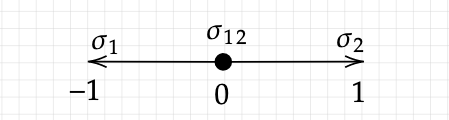
\includegraphics[width=0.8\linewidth]{p1fan.png}
	\end{figure}
	\vspace{1em}

	Although it is outside the scope of the course content, we will conclude by computing the toric variety corresponding to $\Sigma$ to verify it is $\bP^1$. See Fulton pages 3-6 for details. To each cone in $\Sigma$, we associate an affine variety. Note that in this case, $\sigma_1$ and $\sigma_2$ are their own dual cones, and $\sigma_{12}^\vee = \Z$. Thus, $\sigma_1^\vee$ is generated (over $\Z_{\geq 0}$) by $-1=-e_1$, $\sigma_2^\vee$ is generated by $1=e_1$ and $\sigma_{12}^\vee$ is generated by $\{1,-1\} =\{e_1,-e_1\}$. Thus we have
	\begin{align*}
		U_1 &= \Spec(\C[x^{-1}]), & U_2 &= \Spec(\C[x]), & U_{12} = \Spec(\C[x,x^{-1}]).
	\end{align*}
	By definition, we glue $U_1$ and $U_2$ along $U_{12}$. Thus we have the diagram
	\begin{align*}
		\C \rightarrow &~\C^\ast \leftarrow \C\\
		x^{-1} \rightarrow &~x \leftarrow x.
	\end{align*}
	Giving exactly $\bP^1$.

	\subsection{Delzant Polytopes}
	todo 

	\section{Bundles and Divisors}
	\subsection{Line Bundles}
	Let $V=\C^m$, $K = (\C^\ast)^k$, $A=[D_1,...,D_m]$ and $\omega$ be the GIT data for a toric variety $X_\omega$. We will consider line bundles on $X_\omega$ built as quotients of line bundles on $\C^m$. Let $U_\omega$ denote the semi-stable locus of $V$, and consider the trivial line bundle
	$$U_\omega \times \C \to U_\omega$$
	with $K$-action given by $A$ on $U_\omega$ and $d\in \chi(K)$ on $\C$. Kempf's descent lemma tells us that this linearized trivial line bundle descends to form $L_d\to X_\omega$ if the stabilizers of elements in $U_\omega$ act trivially on the fibres of $U_\omega\times \C$. \vspace{1em}

	Example: Let $m=3, k=1$, $A=[1,1,2]$, $\omega=1$, so that $XX_\omega = \bP(1,1,2)$. Then the anti-cones are all non-empty sets: $\cA_\omega = \{I \subset [m] ~|~ I\neq\emptyset\}$. The point $z=[0,0,0,1] \in \C^3$ has stabiliser
	$$K_z = \{t ~|~ [0,0,t^2] = [0,0,1]\} = \{\pm 1\} \cong \Z_2$$
	If we let $U_\omega \times \C$ be linearized by weight $d=1$, then the action of $K_z$ on the fibre at $z$ is non-trivial. However if we pick $d=2$ then the action on the fibre is trivial. Thus the first does not descend to a line bundle, but the second does. \vspace{1em}

	Example: Let $k=2$, $m=5$ and $\omega = [1,1]^T$ and 
	$$A = \begin{bmatrix}
		1 & 0 & 0 & 1 & 1 \\
		0 & 1 & 1 & 1 & 1 \\
	\end{bmatrix}.$$
	Then $[0,0,0,0,z_5,z_6]$ is a semistable point, with stabilizer $K_z = \{(\lambda,\lambda^{-1}) ~|~ \lambda \in \C^\ast\} \subset K$. If we take $d=r[1,1]^T$, then the action of $K_z$ on the fibre is $(\lambda, \lambda^{-1})\cdot l \to \lambda^r\lambda^{-r} l = l$, which is trivial, but for any other linearization the action is non-trivial and the bundle will not descend to $X_\omega$. \vspace{1em}

	Can we find an easier criterion for when a weight will descend to define a line bundle? Observe the stabilizer at some semi-stable element $z$ depends ony on the set $I=\{i ~|~ z_i=0\}$, which corresponds to some $\overline{I}\in \cA_\omega$. This means we should be able to find a condition on anti-cones which tells us if a bundle descends. The stabilizer is the kernel of the map $f_{\overline{I}}:K\to (\C^\ast)^{\overline{I}}$ given by 
	$$\lambda \to (\chi_{D_i}(\lambda))_{i\in\overline{I}}.$$
	Therefore $d\in \chi(X)$ defines a line bundle if $\forall J\in \cA_\omega$, $d(\ker f_J) = \{e\}$. \vspace{1em}
	
	We can rewrite $\ker(f_J) \cong \Z^k/\langle D_i : i\in J\rangle$. The natural surjection $$\Z^k\to \Z^k/\langle D_i : i\in J\rangle$$
	factors through 
	$$\Z^k/\langle d\rangle \Z^k/\langle D_i : i\in J\rangle$$
	if and only if $d\in \langle D_i : i \in J\rangle.$ Therefore
	\begin{prop}
		The bundle $U_\omega\times \C$ linearized by $d\in \chi(K)$ descends to a line bundle on $X_\omega$ if and only if, for all $J\in\cA_\omega$, $d\in \langle D_i ~:~ i\in J\rangle$.
	\end{prop}
	Furthermore, we can convert this into a statement about the fan $\Sigma_\omega$ defining $X_\omega$. Let $\rho_1,...,\rho_n \in M$ be the rays of the fan, and choose a lift of $d\in \chi(K)=\Z^k$ to $\Z^m$. Recall that the map $\Z^m\to Z^k$ is given by the weight matrix $A$, so a lift is equivalent to a choice $(a_1,...,a_m)\in \Z^m$ such that
	$$A(a_1,...,a_m) = \sum_{i=1}^m a_i D_i = d.$$ 
	Associated to such a lift, we can define a map $M\to \Z^m$ by sending $\rho_i\to a_i$. Note that such a map can fail to be well defined. Consider the example of $\bP(1,1,2)$ and linearization $d=1$ from before. From the weight matrix $A$, we can find that the rays of the cone are 
	\begin{align*}
	\rho_1 &= [1,1],& \rho_2 &= [-1,1],& \rho_3 &= [0,-1]
	\end{align*}
	Pick the lift $(1,2,-1)\in \Z^3$. This is a valid lift because $1(1)+2(1)-1(2) = 1 = d$. Then the map $f:M_\R \to \R$ is defined by
	\begin{align*}
		f(\rho_1) &= 1,& f(\rho_2)&=2, & f(\rho_3)&=1.
	\end{align*}
	This is not $\R$-linear. For example, if $f$ was linear, then $\rho_3 = -\frac{1}{2}(\rho_1+\rho_2)$, and hence
	$$f\left(-\frac{1}{2}(\rho_1+\rho_2)\right) = -\frac{1}{2}(f(\rho_1)+f(\rho_2)) = -\frac{3}{2}.$$
	This contradicts that $f(\rho_3)=1$.
	\begin{lemma}
		Let $(a_1,...,a_m)$ and $(b_1,...,b_m)$ be two lifts of $d\in \Z^k$. Let $m_a,m_b:\R^n \to \R$ be the maps defined by $m_a(\rho_i) = a_i$ and $m_b(\rho_i) = b_i$. Then $m_a$ is a linear map if and only if $m_b$ is a linear map.
	\end{lemma}
	\begin{proof}
		By definition, $\sum a_i D_i = \sum b_i D_i = d$. Therefore $\sum (a_i-b_i)D_i =0$, and $(a_1-b_1,...,a_m-b_m) \in \ker(\Z^m \xrightarrow{A} \Z^k)$. By linearity of $A$ this means $m_a\circ A = 0 \iff m_b\circ A =0$. ??? i don't understand
	\end{proof}		
	\begin{prop}
		Let $U_\omega\times \C$ be linearized by a weight $d\in \chi(K)=\Z^k$. This descends to a line bundle on $X_\omega$ if and only if, for all $\sigma_I\in\Sigma_\omega$ and any lift $(a_i)_{i=1}^m$ of $d$, the map $\rho_i\to a_i, i\in I$ defines a linear map. \vspace{1em}

		Equivalently, there exists $m_{\sigma_I} \in M_{\R}$ such that $\langle m_\sigma, \rho_i\rangle = a_i$. 
	\end{prop}
	\begin{proof}
		From the previous proposition, we know the bundle descends if for all $I\in \cA_\omega$, $d\in \langle D_i ~:~ i\in I\rangle$. The cones $\sigma_I$ correspond 1-1 with the anticones $\overline{I}\in \cA_\omega$, so we want to show that 
		$$d \in \langle D_i ~:~ i\in \overline{I} \rangle \iff (\rho_i\to a_i)_{i\in I} \text{ is a linear map.}$$
		If $d\in \langle D_i : i\in\overline{I}\rangle$,  then $d=\sum_{i\in \overline{I}} a_iD_i$ for some $a_i\in \Z$. Therefore letting $a_i = 0$ for $i\in I$, $(a_i)_{i=1}^m$ is a lift of $d$. The corresponding map is the zero map, which is linear. \vspace{1em}
		
		On the other hand, if $d=\sum_{i=1}^1 a_iD_i$ is a lift defining a linear map, then let 
		$$B_I := \begin{bmatrix}
			\rho_{i_1}\\
			\dots\\
			\rho_{i_k}\\
		\end{bmatrix}_{i_j\in I}$$
		The linearity means that
		$$B_I^T \begin{bmatrix}
			b_1\\
			\dots\\
			b_n
		\end{bmatrix}=0 \implies [a_1,...,a_m]\cdot[b_1,...,b_m]=0$$
		I.e. $\ker(B_I^T)\subset\ker([a_1,...,a_m])$. Moreover
		$$\ker(B_I^T) = \text{Im}(A^T) \cap \langle e_i ~|~ i\in I\rangle^T = [\ker(A)+\langle e_i ~|~ i\in I\rangle]^T .$$
		Also, $[a_1,...,a_m]^T \in (\ker A+\langle e_i ~|~ i\in I\rangle)$. Thus $d=\sum a_i D_i = \sum_{k\in I} b_kD_k$, meaning $d\in \langle D_i ~|~ i\in I\rangle$.
	\end{proof}
	\begin{definition}
		An \emph{integral support function} is a continuous map $g:N \to \R$ such that 
		\begin{enumerate}
			\item $g$ is linear on each cone,
			\item $g$ takes integral values on $|\Sigma_\omega|\cap \Z^n$.
		\end{enumerate}
	\end{definition}
	With this definition, the previous proposition says that line bundles over $X_\omega$ are defined by integral support functions on $\Sigma_\omega$. If one drops condition 2, then instead of line bundles one obtains $\mathbb{Q}$-Cartier divisors up to linear equivalence. \vspace{1em}

	Given an integral support function $g$ on a fan $\Sigma_\omega\subset \R^n$, then we can consider the graph of $g$, $\Sigma^g_\omega  \subset \R^n\times \R$. This defines a new fan, with rays $$\{\rho_i' = (\rho_i, g(\rho_i))\}\cup \{\rho_{m+1}'=(\vec{0},1)\}$$ and cones $$\sigma_i\in\Sigma^g_\omega \iff \sigma_{I-{m_1}} \in \Sigma_\omega.$$
	The projection map $\Z^n\times \Z \to \Z^n$ defines a map of fans $\Sigma_\omega^g\to \Sigma_\omega$, and hence induces a map of toric varieties. We claim that the toric variety corresponding to $\Sigma^g_\omega$ is the total space of the line bundle defined by $g$.
	\begin{prop}
		Let $g$ be an integral support function $g$ on a fan $\Sigma_\omega$. Let $X_\omega^g$ be the fan associated to the graph fan $\Sigma^g_\omega$. Then the induced map of toric varieties is a line bundle $X_{\omega}^g\to X_\omega$.
	\end{prop}

	\subsection{Weil and Cartier Divisors}
	Let $X$ be a normal irreducible variety. A prime divisor $D\subset X$ is an irreducible subvariety with codimension 1. Define the sheaf $\mathcal{O}_{X,D}$ by
	$$\mathcal{O}_{X,D}(U) = \mathcal{O}_X(U\cap D).$$
	Then $\mathcal{O}_{X,D}(X)$ is a discrete valuation ring, with valuation $v_D(f)$ equal to the order of vanishing along $D$. Let $\Div(X)$ denote the free abelian group over the prime divisors. 

	\begin{definition}
		A \emph{Weil divisor} is an element of $\Div(X)$. If $D=\sum a_i D_i$, where $D_i$ are prime divisors and all $a_i >0$, then we say $D$ is \emph{effective}.
	\end{definition}
	\begin{definition}
		Let $f \in \mathcal{O}_X$. Then $\Div(f):=\sum_{\text{prime divisors }D}v_D(f)D$. Let $\Div(\mathcal{O}_x):=\Div_0(X)$, called the group of principal divisors. \vspace{1em}

		We say $D_1$ is \emph{linearly equivalent} to $D_2$ or write $D_1\sim D_2$ if $D_1-D_2 \in \Div_0(X)$. 
	\end{definition}
	\begin{definition}
		A Weil divisor is called \emph{Cartier} if it is locally principal. That is, there exists an open cover $\{U_i\}$ of $X$ with $D|_{U_i} = \Div(f_i)$ for some $f_i \in \mathcal{O}_X(U_i)$. We denote the group of Cartier divisors by $\CDiv(X)\subset \Div(X)$. 
	\end{definition}
	\begin{definition}
		The \emph{class group} of $X$ is
		$$\Cl(X) := \Div(X)/\Div_0(X).$$
		The \emph{Picard group} of $X$ is 
		$$\Pic(X) := \CDiv(X)/\Div_0(X).$$
	\end{definition}
	\begin{remark}
		To any Weil divisor $D$ we can associate a coherent sheaf $\OO_X(D)$ by
		$$\OO_X(D)(U) = \{f\in \OO(X) ~|~ \Div(f)+D|_U \geq 0 \}.$$
		If $D_1$ and $D_2$ are linearly equivalent, then $\OO_X(D_1) \cong \OO_X(D_2)$. If $D$ is Cartier, then $\OO_X(D)$ will also be locally free, hence defining a line bundle. This means that $\Pic(X)$ can also be viewed as the group of isomorphism classes of line bundles on $X$.
	\end{remark}
	Now we will restrict our focus back to toric varieties. Let $A=[D_1,...,D_m]$, $K$, $\omega$ be GIT data for a quotient of $V=\C^m$. Let $S=\{i \in [m] ~|~ \{i\}^c \not\in \cA_\omega \}$, and suppose $S=\emptyset$. Consider the set $\{x_i=0\}\cap V^{ss}$. It is closed, $K$ invariant and the image in the quotient will be a prime divisor $\tilde{D}_i$. Now let $T\cong(\C^\ast)^{m-k}$ be the torus inside $X_\omega$, and let $\chi_m\in \chi(T)$. This defines a non-vanishing function $N\to \R$ by $\langle m, \cdot \rangle$. 
	\begin{prop}
		The valuation of $m$ along $\tilde{D}_i$ is given by
		$$v_{\tilde{D}_i}(m) = \langle m, \rho_i\rangle.$$
	\end{prop}
	\begin{proof}
		We can pick a basis of $N$ in which $\rho_i=e_i$. Our assumption that $S=\emptyset$ means that associated to $\rho_i$ is an affine open set $U_i$ corresponding to the anticone $\{i\}^c$;
		$$U_i = \left[
			(\C^\ast)^{\{i\}^c} \times \C^{\{i\}} 
		\right]/K \cong \C\times (\C^\ast)^{n-1}$$
		WLOG we set $i=1$. Then 
		$$U_i = \Spec(x_1,x_2^{\pm},...,x_n^{\pm}).$$
		Let $f\in \C[x_1,...,x_n]$. Then $v_{\tilde{D}_i}(f) = l \in \Z$ and we can write $f=u^l \frac{g}{h}$, with $g/h \in \C[x_2^\pm,...,x_m^\pm]$. We can also write 
		$$\chi^m = \prod_{i=1}^k x_i^{\langle m, r_i\rangle} = x_1^{\langle m, \rho_i\rangle}\prod_{i=2}^k x_i^{\langle m_i, e_i\rangle}.$$
		Letting $f=\chi^m$ and comparing these equations, we see $\langle m_i, e_i\rangle = l = v_{\tilde{D}_i}(\chi^m)$.
	\end{proof}
	\begin{prop}[See CLS]
		Let $\chi^m \in \chi(K)$. Then $\Div(\chi^m) = \sum \langle m, \rho_i\rangle \tilde{D}_i$.
	\end{prop}
	Let $\Div_T(X_\omega)$ denote the $T$-invariant divisors. 
	\begin{exercise}
	Show that $\Div_(X_\omega) = \sum_{i=1}^m \Z \tilde{D}_i$.
	\end{exercise}

\end{document}

